%% LyX 2.3.0 created this file.  For more info, see http://www.lyx.org/.
%% Do not edit unless you really know what you are doing.
\documentclass[12pt,english,a4paper,12pt,openany, marginparwidth=1cm, marginparsep=1cm]{scrbook}
\usepackage[T1]{fontenc}
\usepackage[latin9]{inputenc}
\usepackage[a4paper]{geometry}
\geometry{verbose,tmargin=3.18cm,bmargin=3.18cm,lmargin=4cm,rmargin=2.54cm}
\usepackage{fancyhdr}
\pagestyle{fancy}
\usepackage{xcolor}
\usepackage{babel}
\usepackage{refstyle}
\usepackage{float}
\usepackage{bbding}
\usepackage{amsmath}
\usepackage{amsthm}
\usepackage{amssymb}
\usepackage{graphicx}
\usepackage{wasysym}
\usepackage[numbers]{natbib}
\usepackage[all]{xy}
\PassOptionsToPackage{normalem}{ulem}
\usepackage{ulem}
\usepackage{nomencl}
% the following is useful when we have the old nomencl.sty package
\providecommand{\printnomenclature}{\printglossary}
\providecommand{\makenomenclature}{\makeglossary}
\makenomenclature
\usepackage[unicode=true,
 bookmarks=true,bookmarksnumbered=true,bookmarksopen=true,bookmarksopenlevel=1,
 breaklinks=false,pdfborder={0 0 0},pdfborderstyle={},backref=false,colorlinks=true]
 {hyperref}
\hypersetup{pdftitle={M.Sc Thesis},
 pdfauthor={Yossi Ovcharik},
 pdfsubject={Grasping of Multiple Object with Minimum Fingers},
 breaklinks,linkcolor=black,citecolor=blue, urlcolor=blue}
\usepackage{breakurl}

\makeatletter

%%%%%%%%%%%%%%%%%%%%%%%%%%%%%% LyX specific LaTeX commands.

\AtBeginDocument{\providecommand\figref[1]{\ref{fig:#1}}}
\newcommand*\LyXZeroWidthSpace{\hspace{0pt}}
%% Because html converters don't know tabularnewline
\providecommand{\tabularnewline}{\\}
\RS@ifundefined{subsecref}
  {\newref{subsec}{name = \RSsectxt}}
  {}
\RS@ifundefined{thmref}
  {\def\RSthmtxt{theorem~}\newref{thm}{name = \RSthmtxt}}
  {}
\RS@ifundefined{lemref}
  {\def\RSlemtxt{lemma~}\newref{lem}{name = \RSlemtxt}}
  {}


%%%%%%%%%%%%%%%%%%%%%%%%%%%%%% Textclass specific LaTeX commands.
\theoremstyle{definition}
\newtheorem{example}{\protect\examplename}
\theoremstyle{plain}
\newtheorem{lem}{\protect\lemmaname}
\ifx\proof\undefined\
  \newenvironment{proof}[1][\proofname]{\par
    \normalfont\topsep6\p@\@plus6\p@\relax
    \trivlist
    \itemindent\parindent
    \item[\hskip\labelsep
          \scshape
      #1]\ignorespaces
  }{%
    \endtrivlist\@endpefalse
  }
  \providecommand{\proofname}{Proof}
\fi
\theoremstyle{plain}
\newtheorem{prop}{\protect\propositionname}
\theoremstyle{definition}
\newtheorem{defn}{\protect\definitionname}

%%%%%%%%%%%%%%%%%%%%%%%%%%%%%% User specified LaTeX commands.
% Algorithms
\usepackage[linesnumbered,algoruled,boxed]{algorithm2e}
%\PassOptionsToPackage{linesnumbered}{algorithm2e}
%\PassOptionsToPackage{algoruled}{algorithm2e}
%\PassOptionsToPackage{boxed}{algorithm2e}

% set fonts for nicer pdf view
\IfFileExists{lmodern.sty}{\usepackage{lmodern}}{}
%\usepackage{myModule}

\DeclareMathOperator*{\argmax}{argmax}
\DeclareMathOperator*{\argmin}{argmin}



\newcommand*{\blankpage}{%
  \par\vspace*{0.25\textheight}%
  {\centering \emph{This page intentionally left blank.}\par}
  \vspace{\fill}%
}
\usepackage{scrlayer}
\DeclareNewLayer[
    foreground,
    textarea,
    contents=\blankpage
  ]{blankpage.fg}
\DeclarePageStyleByLayers{blank}{blankpage.fg}
\KOMAoptions{cleardoublepage=blank}


% Allow nomenclature entries with units
\newcommand{\nomunit}[1]{%
% \renewcommand{\nomentryend}{\hspace*{\fill}#1}}
\renewcommand{\nomentryend}{\dotfill#1}}


% avoids that floats are placed above its sections
%\let\mySection\section\renewcommand{\section}{\suppressfloats[t]\mySection}

% Use this for naming ref types when referencing.
\providecommand{\thmautorefname}{Theorem}
\providecommand{\corautorefname}{Corollary}
\providecommand{\lemautorefname}{Lemma}
\providecommand{\propautorefname}{Proposition}
\providecommand{\eqautorefname}{Equation}


\usepackage{subfig}
\newcommand{\subfigureautorefname}{\figureautorefname}


% Make references automatically formatted
\AtBeginDocument{%
\let\ref\autoref
%\renewcommand\equationautorefname{\@gobble}
}



% Flowcharts
\usepackage{tikz}
\usepackage{pgfplots}
\usepackage[siunitx]{circuitikz}
\usetikzlibrary{shapes,arrows,matrix}
\usepackage{pgfplots}
\usepackage{smartdiagram}

\@ifundefined{showcaptionsetup}{}{%
 \PassOptionsToPackage{caption=false}{subfig}}
\usepackage{subfig}
\makeatother

\def\eqdeclaration#1{, see equation\nobreakspace(#1)}
\def\pagedeclaration#1{, page\nobreakspace#1}
\def\nomname{Nomenclature}
\providecommand{\definitionname}{Definition}
\providecommand{\examplename}{Example}
\providecommand{\lemmaname}{Lemma}
\providecommand{\propositionname}{Proposition}

\begin{document}
\global\long\def\reals{\mathbb{R}}
\global\long\def\rthree{\reals^{3}}
\global\long\def\rsix{\reals^{6}}
\global\long\def\rtwo{\reals^{2}}

\global\long\def\x{\times}

\global\long\def\z#1{\textbf{*\textcolor{red}{\emph{*\;#1}}} }

\global\long\def\zz#1{\textsf{\textbf{\textit{*\textcolor{red}{\emph{*\;#1}}}}} }

\pagenumbering{gobble}

\subject{Ben-Gurion University of Negev\\
Faculty of Engineering Sciences\\
Department of Mechanical Engineering\\
$\hfill$\\
\includegraphics[width=0.15\paperwidth]{images/BGU_Logo}}

\title{SIMULTANEOUS GRASPING OF MULTIPLE OBJECTS}

\subtitle{\vspace{0.15\textheight}
}

\author{A thesis submitted in partial fulfillment of\\
 the requirements for the degree of Master of Science\\
\\
by Yosef Ovcharik\\
Advisor: Prof. Amir Shapiro}

\date{July 2018}
\maketitle

\minisec{Abstract}

kfkfasjkdklsfaja sdfl;afjl;asdf
\begin{center}
\textbf{\vspace{0.25\textheight}
}
\par\end{center}

\begin{flushleft}
{\large{}Prepared by: Yosef Ovcharik}{\large{}\uline{\qquad{}\qquad{}\qquad{}\qquad{}}}{\large\par}
\par\end{flushleft}

\begin{flushleft}
{\large{}Advisor: Prof. Amir Shapiro}{\large{}\uline{\qquad{}}}{\large\par}
\par\end{flushleft}

\chapter*{Acknowledgments}

I am very grateful to my arms for being by my side, to my legs for
carrying me, and to my fingers - I can always count on them.

\frontmatter

\fancyhf{}
\fancyhead[LE]{\leftmark }
\fancyhead[RO]{\rightmark}
\fancyfoot[LE,RO]{\thepage}

\addcontentsline{toc}{chapter}{Contents} % TOC to appear in TOC

\tableofcontents{}

\listoftables

\addcontentsline{toc}{chapter}{List of Tables} % Puts toc item link to THIS place

\listoffigures

\addcontentsline{toc}{chapter}{List of Figures}

\settowidth{\nomlabelwidth}{$p_{c_{i}}$}
\printnomenclature{}

\addcontentsline{toc}{chapter}{Nomenclature}

\begin{table}[tbh]
\centering{}%
\begin{tabular}{|c|c|c|}
\hline 
\multicolumn{2}{|c|}{\textbf{Task}} & \textbf{Status}\tabularnewline
\hline 
\hline 
\emph{Preliminaries} & \emph{Background} & \Checkmark{}\tabularnewline
\hline 
 & \emph{Related work} & \Checkmark{}\tabularnewline
\hline 
 & \emph{Definitions} & \Checkmark{}\tabularnewline
\hline 
 & \emph{Assumptions} & \Checkmark{}\tabularnewline
\hline 
 & \emph{Problem Statement} & \Checkmark{}\tabularnewline
\hline 
\emph{Solution} & \emph{Description} & \Square{}\tabularnewline
\hline 
 & \emph{Limitations} & \Square{}\tabularnewline
\hline 
 & \emph{Algorithm} & \Square{}\tabularnewline
\hline 
 & \emph{Complexity} & \Square{}\tabularnewline
\hline 
\emph{Simulations} & \emph{Software} & \Square{}\tabularnewline
\hline 
 & \emph{Setup} & \Square{}\tabularnewline
\hline 
 & \emph{Results} & \Square{}\tabularnewline
\hline 
\emph{Experiments} & \emph{Setup} & \Square{}\tabularnewline
\hline 
 & \emph{Results} & \Square{}\tabularnewline
\hline 
\emph{Discussion} &  & \Square{}\tabularnewline
\hline 
\emph{Conclusions} &  & \Square{}\tabularnewline
\hline 
\emph{Introduction} &  & \Square{}\tabularnewline
\hline 
\emph{Abstract} &  & \Square{}\tabularnewline
\hline 
\emph{Title} &  & \Checkmark{}\tabularnewline
\hline 
\emph{Acknowledgments} &  & \Square{}\tabularnewline
\hline 
\emph{References} &  & \Checkmark{}\tabularnewline
\hline 
\end{tabular}\caption{Advancement.}
\end{table}

\mainmatter


\chapter{Introduction}

\section{Motivation {[}1 page{]}}

Robotics become a vast field of research and applications,
\begin{itemize}
\item Technologies
\item Robotic manipulators
\item Grasping
\item Automation
\item Home Assistance
\item Defense applications
\item Remote robotics (space etc.)
\end{itemize}

\section{Research objectives {[}.5-1 page{]}}

While vast amount of research is done on grasping in different forms
(manipulators, fixturing, first\textbackslash second order, machine
learning approach, visual assessment, restraint analysis etc.) little
work was done on grasping/manipulation of several objects an once.

The main objective of the research is to present a solution for immobilization
of several objects simultaneously, while using minimal amount of actuators
(fingers). That can be achieved by analyzing the spatial relationship
of objects and the contacts between them.

The research can be divided to sub-objectives:

Classifying the types of contacts between bodies.

Assessment of additional constraints needed to immobilize the set
of objects

Deriving an optimal way to arrange the objects in order to minimize
the amount of external constraints needed for the immobilization.

\section{Research contribution and innovation {[}.5-1 page{]}}

The research yielded solid and reproducible results of multiple object
immobilization that can be integrated in various robotics systems.

The methods described are novel solutions for the problems yet to
arise.

The research can be further extended to manipulation of multiple objects,
interaction with soft objects / fingers and, of course, all of this
in 3D space.

Some of the products of the research can be used for more intelligent
manipulation in cases where variety of items exist and decisions as
to selection of groups to be moved simultaneously have to be made.
Example of such use: home assistance robotic system that performs
a task of sorting and storage of groceries.

Should mention ICRA here, and the book that could be published.

\section{Literature Review\label{sec:Literature-Review}}

Important contribution to the future development of robotics in general
and grasping in particular belongs to \citet{Reuleaux1876,Landau1982}
for bringing the basics of mechanics and mechanism kinematics, which
serve as foundation for every analytical approach of robotics study.
\citet{Lozano-Perez1983} for the introduction of Configuration Space
use which contributed in vast majority of fields. Use of the Configuration
Space representation has been a major interest for the simultaneous
multi-body manipulation, yet because of high computation cost and
lack of explicit analytical formulations was not fully incorporated
in this research.

\citet{Ball1998} introduces an essential ideas of screw theory which
allows use of wrench and wrench space concepts, tools that take major
part in the contemporary robotics. \citet{Murray1994} presents concise
and yet thorough survey on appliance of the mathematical tools for
the description of manipulations. With general tools for mechanisms
and manipulators in particular, interaction of such manipulators with
the environment can be formulated using Coulomb's friction, categorizing
contacts for frictional, frictionless, hard or soft contacts \citet{Murray1994}.
\citet{Rimon1995} proposed bounds on number of frictionless fingers
for 2D polygonal object immobilization.

Given broad mathematical basics, grasping becomes of particular interest
with \citet{Mishra1987} showing existence of positive grasps, and
allowing following grasp synthesis development: \citet{Bunis2018,Borst2004}.
Derivations would not be possible without defining form and force
closure by \citet{Asada1989}\citet{Rimon1996}. \citet{Nguyen1986}
proposes a viable methods for constructing force closure grasps.

More methods on grasp construction include synthesizing grasps evolved
from predefined configurations \citet{Pollard1996}, mimicking human
behavior in grasping tasks: using predefined shapes and modes for
closure grasps are planned with numerical computations of trajectories
intersections \citet{Wren1995}.

Contact modeling \citet{Xydas1999}

\citet{Rimon1998} propose a novel idea of mobility index based on
second order curvature of bodies in contact, intended for multi-finger
grasping.

Grasp evaluation takes a long way with \citet{Mishra1989} discussing
the stability of grasps, \citet{Ferrari1992} introducing quality
measures based on wrenches, \citet{Roa2015} surveying several methods
of grasp quality measure, while\citet{Lin1997} extend the measures
for complaint grasps.

Grasp generation can be addressed with different approach, with randomized
grasp generation\citet{Borst2003} where grasp candidates are generated,
tested for force closure and evaluated according to desired quality
measures.

Integrating methods in real life applications usually require use
of vision systems as shows\citet{Corke2011} and often extended to
use of machine learning for vision based grasping:\citet{Quillen2018,Bezak2014,Le2010}.

The list would not be full without mentioning\citet{Siciliano2016}
providing an overview and composition of concepts and techniques in
grasp synthesis, evaluation and optimization.

Most methods for grasp construction are searching for force closure
grasps, some of them for optimal grasps. Usually the complexity of
the computations depends on the number of edges / faces of the object
to be grasped.

Multiple objects grasping\citet{Pajarinen2017,Zeng2017}

\z{Put more info on CONFIGURATION SPACE approach to grasping}

What about Stable pushing of stacked parts

\section{Preliminary Background}

Basically this part should explain to the reader all the basics that
are known prior this work. Everything that is out of the scope of
the B.Sc in mechanical engineering should be addressed and explained.

Starting with introduction to grasping, contact models and grasp matrix,
follow with for closure and form closure, grasp planning (fingers
number, conditions and grasps). Restraint analysis (form closure).
Need to describe: workspace, closure, contacts, twist and wrench duality.

Notation in robotics makes a wide use in vectors and matrices, along
with coordinate frames and transformations. A lot of concepts are
drawn from linear algebra.

Manipulator forces, relations between joint forces/torques and end-effector
forces, singularities, dynamics of manipulators etc. is out of the
scope of this work.

\z{Convex cones and dual cones}

\subsection{Motion and Forces}

Traditionally, motion of rigid bodies can be described by utilizing
a concept knows as twist: the description of both linear and angular
velocities of a rigid body.\citet{Murray1994} shows that any rigid
body motion can be described using a twist, namely that every motion
of a rigid body can be described by a rotation of a body about an
axis and translation of that body in direction parallel to that axis
-- known as\emph{screw} motion. The mapping between twist and screws
can be done using matrix exponential.
\begin{equation}
V=\begin{bmatrix}\upsilon\\
\omega
\end{bmatrix}\in\rsix\qquad\upsilon\in\rthree,\,\omega\in\rthree
\end{equation}
A generalized force, acting on the body is described as a\emph{wrench}-
force/moment pair, which consists from a linear component and an angular
component acting on a point.
\begin{equation}
F=\begin{bmatrix}f\\
\tau
\end{bmatrix}\in\rsix\qquad f\in\rthree,\,\tau\in\rthree
\end{equation}
Combination of wrench and twist define power: the dot product of twist
and wrench yield instantaneous power. Reciprocal wrenches and twist
are combinations that have instantaneous zero power:$F\cdot V=0$.
Both concepts can be described as screws, and this way threat them
in same way. The notion allows simple analysis of kinematics of mechanisms
in general, and, more importantly, grasping in particular.

In grasping, the wrenches applied to the object act as a set of constraints,
and twists are possible motions of the object. If acting wrenches
allow no reciprocal twists, i.e. there is no twist that for every
wrench the dot product will be 0, then the object is immobilized.

\subsection{Grasping and Immobilization}


\subsubsection*{Contacts}

Basic concept in grasping is a contact between a finger and an object.
Contact describes the mapping of forces applied by fingers at some
point on the object boundary to resultant wrenches in object coordinate
frame. A set of properties should be defined for a contact:
\begin{itemize}
\item Contact point location
\item Contact type
\item Forces and torques applied by the contact
\end{itemize}
Contact point location is usually defined in object-attached coordinate
frame. It is convenient to define the origin of this coordinate frame
at object's center of mass, and to set contact coordinate frame where\emph{z-axis}
is normal to the object surface, pointing inside of the object, this
way positive\emph{z} value means pressure applied by a finger. Term
pressure here means that finger can exert only pressing force and
not pulling, as opposed to suction cups.\ref{fig:Coordinate-frames}
illustrates coordinate frames:\emph{$O$} - object coordinate frame,\emph{$C$}
- contact coordinate frame together with vector$r_{c}$ which defines
the location of contact point in object coordinate frame.\nomenclature{$r_{c}$}{distance between coordinate systems origins \nomunit{[mm]}}
\begin{figure}[tbh]
\noindent \centering{}\includegraphics[width=0.25\textwidth]{\string"images/object w contact\string".eps}\caption{\label{fig:Coordinate-frames}Coordinate frames.}
\end{figure}
Contact type would describe the interaction between the surface of
the object and the surface of the finger. Common cases are: normal
force only, in cases where friction coefficient is low; normal and
tangent forces, in cases where friction is significant; normal and
tangent forces along with normal torque (torsional friction). Typical
examples for given contact types are: pressing a pen tip against a
glass - normal force only; pressing a pencil tip against rubber -
can provide normal and tangent forces; pressing a hand against a paper
sheet laid on a table: friction coefficient between a sheet and a
table is considerably lower than this between the hand and the sheet,
this way we could move the sheet aside and rotate it about axis normal
to the table surface.

\subparagraph*{Frictionless point contact}

is a simplest type of contact which can apply forces only in the direction
of the surface inward normal.

\subparagraph{Point contact with friction}

is a more realistic contact which can apply both normal and tangent
forces on an object. The modeling of a friction between a finger and
an object surface could be simplified by assuming that the finger
can exert small tangent forces, linearly depended with a normal force.
This would produce a\emph{friction cone} as shown in\ref{fig:Friction-cone}.
Normal force\nomenclature{$f_{n}$}{normal force \nomunit{[N]}} and
tangent force\nomenclature{$f_{t}$}{tangent force \nomunit{[N]}}
written as$f_{n}$ and$f_{t}$ respectively. Tangent force depends
on normal force. and thus can be described mathematically by inequality:
\begin{equation}
\begin{gathered}f_{t}\leq f_{n}\cdot\mu\end{gathered}
\end{equation}
where$\mu$ stands for coefficient of friction\nomenclature{$\mu$}{coefficient of frfiction}
between a finger and a surface. For practical applications, friction
cone is approximated by finite set of vectors lying on cone's lateral
surface. In 2 dimensional space it takes a form of an isosceles triangle
with a vertex between two equal edges located at the contact point,
and the bisector lies along the normal direction. The half angle of
the aforementioned vertex is defined by$\alpha=\arctan\left(\mu\right).$

\begin{figure}[tbh]
\noindent \centering{}\includegraphics{\string"images/friction cone\string".eps}\caption{\label{fig:Friction-cone}Friction cone.}
\end{figure}


\subparagraph{Soft finger}

is the most``capable'' contact, able to apply both normal and tangent
forces, and a torque about the contact normal as well. In$\rtwo$
the concept is not used since rotations only possible around 1 axis.

\z{INSERT CONTACT TYPES SUMMARIZING FIGURE HERE}

\subsubsection*{Grasp and Grasp Matrix}

A grasp is a collection of contacts (types and locations) that can
apply forces and torques on a body. Contact forces applied to the
object will result in a resulting force and torque - wrench. A matrix
transforming contact wrenches to object wrenches can be derived from
contact locations and types, and forces applied. Construction of the
grasp map can be automatized for accurately known objects and fingers.
Derivation of the matrix is not shown here, reader can refer to\citet{Murray1994}
for more detailed explanation.

\textcolor{brown}{\z{MAYBE IT SHOULD BE SHOWN HERE.\\
GM maps the contact forces at contact locations to wrenches induces in the body.
}}
\begin{example}
Grasp map derived by\citep{Murray1994} p.222 is presented below in\ref{fig:Planar-grasping}:
a planar rectangular object held by two fingers which apply forces
in the plane. Resulting wrench on the object from one finger can be
described as following:
\begin{equation}
F_{o}=\begin{bmatrix}f_{o}\\
\tau_{o}
\end{bmatrix}=\begin{bmatrix}R_{c} & 0\\
\begin{bmatrix}-p_{y} & p_{x}\end{bmatrix}R_{c} & 1
\end{bmatrix}\cdot\begin{bmatrix}f_{c}\\
\tau_{c}
\end{bmatrix}
\end{equation}
where$R_{c}$ represents\z{WHAT?}. Grasp map for this example is
given by:
\begin{equation}
G=\begin{bmatrix}0 & 1 & 0 & -1\\
-1 & 0 & 1 & 0\\
r & 0 & r & 0
\end{bmatrix}.\label{eq:GraspMap}
\end{equation}
\begin{figure}[tbh]
\noindent \centering{}\includegraphics[width=0.75\textwidth]{images/Murray-GraspMap}\caption{\label{fig:Planar-grasping}Planar grasping.}
\end{figure}
Although the derivation of the grasp matrix is not shown here, reader
can intuitively see that locations of contacts and orientation of
contact coordinate frames are reflected in this representation. Using
grasp map, total wrench on the object could be defined as:
\end{example}
\nomenclature{$F_{o}$}{wrench vector \nomunit{[N and Nmm]}}\nomenclature{$f_{c}$}{contact force vector \nomunit{[N]}}\nomenclature{$f_{c}$}{contact force vector \nomunit{[N]}}\nomenclature{$f_{i}^{j}$}{$i$-coordinate component of $j$ contact force \nomunit{[N]}}\nomenclature{$r$}{contact location distance from origin \nomunit{[mm]}}\nomenclature{$G$}{\nomunit{[unitless]} grasp map matrix}
\begin{equation}
F_{o}=G\cdot f_{c}=\begin{bmatrix}0 & 1 & 0 & -1\\
-1 & 0 & 1 & 0\\
r & 0 & r & 0
\end{bmatrix}\cdot\begin{bmatrix}f_{x}^{1}\\
f_{y}^{1}\\
f_{x}^{2}\\
f_{y}^{2}
\end{bmatrix},
\end{equation}
 where$F_{o}$ denotes a total wrench (force and torque combined)
applied to the object,$G$ is the grasp map as shown in\ref{eq:GraspMap}
and$f_{c}$ is contact forces vector (normal and tangent forces applied
by each and every finger). Expanding the matrix-vector product yields
total wrench that can be confirmed by visual observation of\ref{fig:Planar-grasping}:\nomenclature{$F_{i}$}{force component in $i$ direction \nomunit{[N]}}\nomenclature{$T_{i}$}{torque component in $i$ direction \nomunit{[Nmm]}}
\begin{equation}
\begin{bmatrix}F_{x}\\
F_{y}\\
T_{z}
\end{bmatrix}=\begin{bmatrix}f_{y}^{1}-f_{y}^{2}\\
-f_{x}^{1}+f_{x}^{2}\\
r\cdot f_{x}^{1}+r\cdot f_{x}^{2}
\end{bmatrix}.
\end{equation}
The space that is spanned by all contacts is called the Grasp Wrench
Space (GWS) and characterizes the ability of the grasp to balance
disturbance forces. A convex hull of vectors from grasp matrix rows
with torque values normalized with some reference distance (radius
of a sphere with same volume as the grasped object, for example) can
be further used to analyze the grasp quality.

\subsubsection*{Grasp properties:}

Given a grasp one can inquire what are the properties of that grasp,
how good is it and whether it is suitable for desired task:
\begin{labeling}{00.00.0000}
\item [{Equilibrium~grasp}] is a grasp where fingers can exert forces
that will keep the grasped object in the equilibrium state.
\item [{Manipulability}] defines whether arbitrary motions of a grasp object
can be generated by applying forces by the fingers.
\item [{Immobilization}] grasp is called immobilizing if applied contacts
prevent any motion of the object (translation or rotation).
\item [{Grasp~redundancy}] the grasp can consist of number of fingers,
while not every one of them is necessary (e.g. for immobilization,
or for equilibrium grasp).
\item [{Grasp~stability}] Presented by\citet{Montana1988}.\citet{Bicchi2000}
summarized that the grasp stability depends on the local geometry
of the grasp body. One of the definitions of stability is based on
the potential function of the contacts forces, and the grasp said
to be stable if for small perturbations from the equilibrium grasp
the potential function has positive gradient, and unstable otherwise.\\
Extension (or reduction) of grasp stability on contact stability can
be described as follows: If two bodies are in contact and are held
in equilibrium by external forces (e.g. fingers), if for small perturbation
of contact position, the contact will stay in that new position or
return to the original position than the contact is stable. More detailed
explanation presented in the\ref{subsec:Relationship-between-polygons}
.
\end{labeling}

\paragraph*{Force Closure}

A grasp is a force closure if the space of object wrenches is spanned
by the set of finger forces and include the origin surroundings inside
the convex hull of applied wrenches.

If a grasp can resist any external wrench applied to the object the
grasp is called\emph{force-closure}. One way to ensure that given
grasp is force-closure is constructing\emph{convex hull}. If convex
hull contains the origin then the grasp is force closure.

Constructing of convex hull is done by using the columns of grasp
map: each column represents a vector. Plotting these vectors and closing
polygons between them will yield a convex hull shape (polyhedron).
Normally tangent forces are result of friction and along with normal
forces can be defined by cones, as shown above. For the matter of
simplicity of the example, tangent forces are assumed to be independent
of normal once. Hence,$f_{x}$ assumed to be positive or negative,
where$f_{y}$ is positive only as shown in\ref{fig:Convex-hull} .
\begin{figure}[tbh]
\noindent \begin{centering}
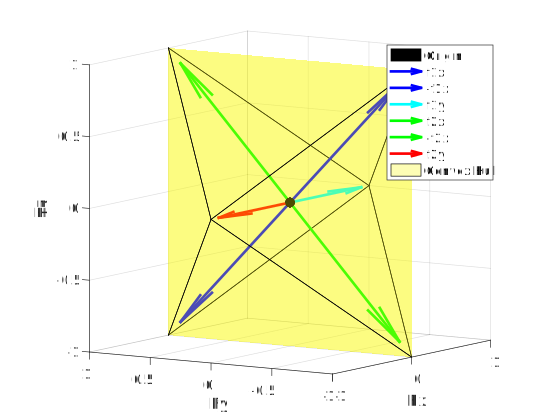
\includegraphics[width=0.5\textwidth]{images/ConvexHull}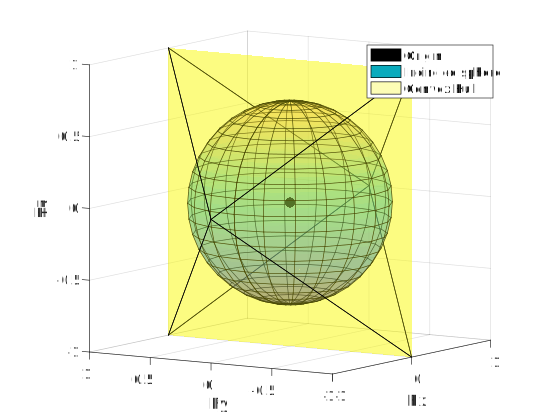
\includegraphics[width=0.5\textwidth]{images/ConvexHull-Sphere}
\par\end{centering}
\caption{\label{fig:Convex-hull}Convex hull (left) and inscribed sphere (right).}
\end{figure}
Once convex hull is built, quantitative assessment can be performed.
One way of doing that is determining the largest sphere to inscribe
in the hull with its center at origin, as shown in\ref{fig:Convex-hull},
and measuring it's diameter. If vectors are normalized, the radius
of the sphere can serve as\textbf{\emph{grasp quality measure}}(dimensionless
value)\emph{.} In case of 3-dimensional space and object convex hull
is 6-dimensinoal:$F_{x},F_{y},F_{z},T_{x},T_{y},T_{z}$ and it cannot
be shown fully in 3-dimensinal domain, but projections such as$F_{x},F_{y},F_{z}$
can be presented.

\paragraph*{Form Closure}

A grasp is a form closure if it is a force closure and the fingers
are frictionless contacts. The form closure is``geometrical'' immobilization
of an object, discarding friction forces etc.

Form closure: Constrain the movement of the object

\z{INSERT IMAGES ON FORM AND FORCE CLOSURE, EQUILIBRIUM GRASP, MANIPULABLE GRASP}

\subsubsection*{Quality Measures}

\textcolor{brown}{\z{NEED MORE INFO HERE}}

{[}Ferrari and Canny{]}\citep{Ferrari1992} Radius of largest hyper-sphere
you can fit in convex hull centered in origin

{[}Zhu and Wang{]}: Numerical test which measures the scaling factor
for the maximum compact set incribedin the grasp wrench space

Quantifying the quality of the grasp. Task Wrench Set. Inscribed sphere.\citet{Borst2004,Roa2015}

\subsubsection*{Grasp planning and construction}

When planning a grasp for given object, one has to determine how many
contacts and of what kinds are needed.\citet{Murray1994} reminds
that for spatial object, 4 friction contacts are sufficient for grasp.
But, when dealing with robotic grippers, contact locations are limited
due to gripper geometry, and forces gripper can apply are limited
too. Given an object and a multifingered robot hand (along with robot
itself) maximal wrenches an hand can exert can be calculated. Xiong
et al. (2007)\citep{Xiong2007} shows extended grasp capability assessment,
but for the purposes of this research it is safely to assume that
the objects are light enough and the hand is robust enough to exert
desired wrenches. Yet contact locations are limited because of the
dimensions of finger and placement of the fingers on the palm (e.g.
opposing finger vs symmetric pattern).

Variety of methods for grasp planning was presented during years,
yet for the purposes of this research we use geometrical methods as
proposed by\citet{Nguyen1986}. The paper shows that for construction
of force closure grasp with 4 planar forces only, the geometric necessary
and sufficient condition is that that no more than 2 force directions
does not intersect in one point, and remaining 2 force directions
result in moments with different signs about the aforementioned intersection
point.\z{INSERT NEW IMAGES}:

\begin{figure}[tbh]
\noindent \begin{centering}
\includegraphics[width=0.3\textwidth]{images/nguyen_1}\includegraphics[width=0.3\textwidth]{images/nguyen2}
\par\end{centering}
\caption{NGUYEN}
\end{figure}
The methods uses geometric relations between object's edges and corresponding
normal directions to construct polygons and determine edge regions
suitable for finger placement. Method can be used both for frictional
and frictionless contacts (2 fingers needed for frictional grasp).

Additional method that is used in a research is random grasp generation
with evaluation of the resultant grasps, as proposed by\citet{Borst2003}.
Main idea is to generate random contact points along the object's
boundary and evaluate the resultant grasp both for force closure and
for given quality measure.

Find optimal set of graphs with independent regions of contact and
pick mid points of the regions as optimal grasp points.

\subsection{Graphs}

\textcolor{brown}{\z{Rethink this section}}

The main interest of this research is multiple objects grasping which
requires objects interaction classification. Some of the objects can
be in contacts with other object(s) and these connections will be
partially described by a graph.

Graph is structure describing a set of objects and relations between
them. In case when every pair of nodes in graph are connected the
graph is called Connected Graph. Undirected graphs alone are the utilized
in this work. Adjacency matrix is a way to represent a finite graph.
For non-directed graphs the adjacency matrix is symmetric. Matrix
elements indicate whether a connection exists between 2 nodes, and
also may quantify the connection.

\z{EXAMPLE GRAPHS, ADJACENCY MATRICES}

\section{Assumptions}

This work focuses on planar space where objects represented as polygons
with finite amount of edges. Knowledge of exact location and orientation
of those polygons are assumed, along with the knowledge of the exact
shape.

The polygons are assumed to be non-self-intersecting, while for practical
purposes the null-thickness regions of self-intersection polygons
can be infinitesimally thickened to form a non-self-intersection polygon.

In a given set of objects only connected configurations are of interest.
The problem with more than one distinct group of connected polygons
are easily divided to subproblems.

The work focuses on construction of equilibrium force closure grasps
with frictionless fingers using first order geometry (i.e. form closure).

Finger contacts are point contacts and hence can act on one object
at a time, two fingers cannot be placed at same location.

\section{Problem Statement}

\z{What should be written here at all? Do I need this section? Probably I do, check Yoav's thesis, and Amir's and Avishay's as well.}
\begin{description}
\item [{Given:}] A set of polygonal objects in 2D space.
\item [{Desired:}]~
\begin{description}
\item [{A}] Configuration of objects in space achieved by translation and
rotation only (no reflections).
\item [{B}] Minimal set of finger locations to immobilize all of the given
objects.
\end{description}
\end{description}

\chapter{Proposed solution}

In a common workspace polygonal objects can contact one another in
several ways. Classification of the relations between the polygonal
allows more thorough state analysis and further planning. After the
classification is presented, an algorithm for finger placement given
configuration of polygons is proposed, and then an algorithm for polygons
placement is proposed.

\z{The idea can be expanded for various tasks, such as home assistant robot that brings several items in one run.
 This should go to Motivation.}

Thus, the solution can be subdivided into 2 parts: determining the
minimal amount and placement of fingers required to immobilize given
set of contacting polygonal objects and a determination of desired
configuration (rearranged set of objects) that will require minimal
amount of finger to immobilize it. Both parts require examination
of inter-object contacts and relations between objects, along with
classification for further analysis.

\begin{figure}[tbh]
\noindent \begin{centering}
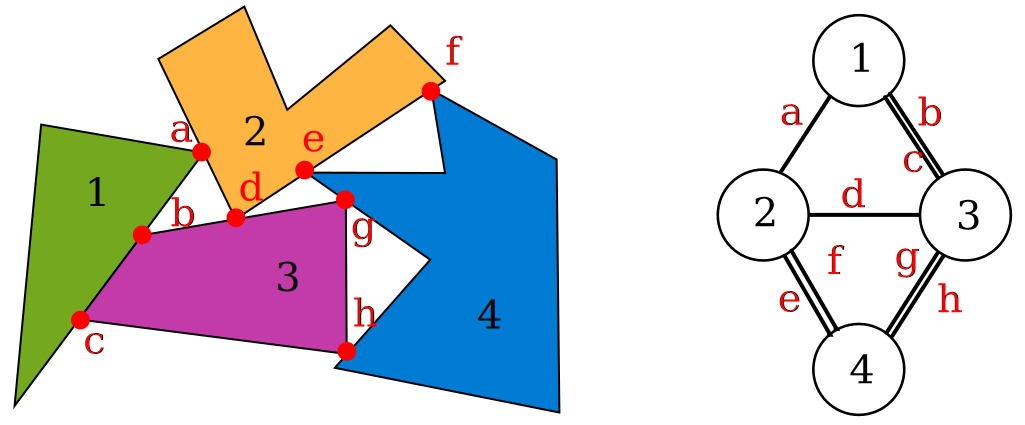
\includegraphics[width=0.7\textwidth]{images/set_example}
\par\end{centering}
\caption{Objects set and a corresponding graph.\label{fig:Objects-set-and}}
\end{figure}

\begin{example}
4 objects in\ref{fig:Objects-set-and} where 1 and 2 touch 3, and
4 touches 2,3. The contacts serve as graph edges, while objects are
represented as graph nodes. Graph for the given object configuration
is shown below. Adjacency matrix describing given graph is presented:
\[
A=\begin{bmatrix}0 & 1 & 2 & 0\\
1 & 0 & 1 & 2\\
2 & 1 & 0 & 2\\
0 & 2 & 2 & 0
\end{bmatrix}.
\]
General idea is to find an amount of missing finger contacts for each
object and each set of objects by examining the relationship between
them.
\end{example}

\section{Mathematical description}

REWRITE THIS SECTION\footnote{Treat the contact point and not the whole polygon. Think what do I
want to say here at all.}

Given 2 polygons,$p_{1},p_{2}$. The twist of polygon$p_{1}$ relative
to$p_{2}$ can be defined as$\dot{x}_{12}=\left(v_{12},\omega_{12}\right)^{T}$.
Polygons can maintain contact but not penetrate one another.

\z{Let $IP$ denote the set of interaction points common to both polygons.
Let $C=\left\{ c_{i}\right\} $ be a set of contact descriptions between these polygons. } 

Let$\hat{n}_{i}^{j}$ denote the inward normal direction of the boundary
of polygon\emph{j} at contact point\emph{i}.

The contact between the polygons can be described using one or more
contact points and corresponding contact normal directions.

\subsection{Relationship between polygons and polygon sets\label{subsec:Relationship-between-polygons}}

The examination of given polygon configuration can be subdivided to
interaction of each couple of polygons. The polygons can be disconnected
- no points belong to 2 polygons simultaneously, or connected - one
ore more points belong to 2 or more polygons. The connection between
the polygons can be represented by a contact description. A stable
contact between 2 polygons can exist in several variants:
\begin{labeling}{00.00.0000}
\item [{\textbf{Vertex-Edge}}] Vertex to edge contact is the discrete contact
where a vertex of the first polygon ($p_{1}$) is coincident with
an edge of the second polygon ($p_{2}$). The contact normal direction
is defined by the edge the of the second polygon. The set of contacts
for this variant consists of a single contact:$C=\{c_{1}\}.$ Contact
restrictions can be described as following: velocity of the contact
point on the boundary of$p_{1}$ relative to the velocity of the contact
point on the boundary of$p_{2}$ (denoted$v_{12}$) cannot have component
in direction$\hat{n}_{1}^{2}$ - polygons cannot penetrate. This can
be expressed as follows:$v_{12}\cdot\hat{n}_{1}^{2}\leq0$. Contact
is maintained when the component of the relative velocity in the direction
if inward normal of first polygon is 0. Since$\hat{n}_{i}^{2}=-\hat{n}_{i}^{1}$,$-v_{12}\cdot\hat{n}_{1}^{2}\leq0$.
Therefore, the contact is maintained when relative velocity of contact
points of each polygon are perpendicular to the edge normal.
\begin{equation}
v_{12}\cdot\hat{n}_{1}^{2}=0
\end{equation}
\begin{figure}[tbh]
\noindent \begin{centering}
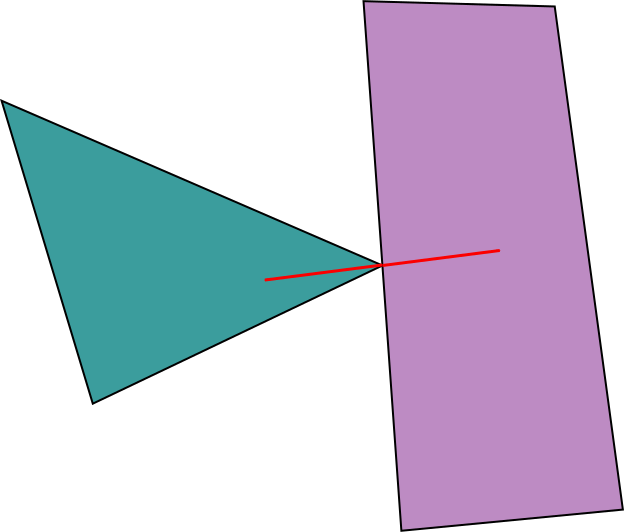
\includegraphics[width=0.35\textwidth]{images/cont_v2e}
\par\end{centering}
\caption{Vertex-to-Edge contact example.}
\end{figure}
\item [{\textbf{Edge-Edge}}] Edge to edge contact is a continuous contact
between two bodies along a continuous segment. Since the edges are
finite, there exist at least 2 vertices belonging to either one or
two polygons that belong to the contact segment. In a way analogous
to distributed load concentrated in a point, the continuous distributed
contact can be concentrated in 2 different points. Two different vertices
are selected to be such points. Since the vertices lie along the same
edge, the contact normal directions are the same in this case. The
set of contacts for this variant consists of two contacts:$C=\{c_{1},c_{2}\},\;c_{i}=\left\{ r_{i},\hat{n}\right\} $,
where$r_{i}$ stands for contacts' location and$\hat{n}$ stands for
the normal direction of the edge. Graphically this can be depicted
as follows: Polygon 1, polygon 2, contact line, contact points. Cases
with 2 points, case with 3 vertices, case with 4 vertices in contact.
\begin{figure}[tbh]
\noindent \begin{centering}
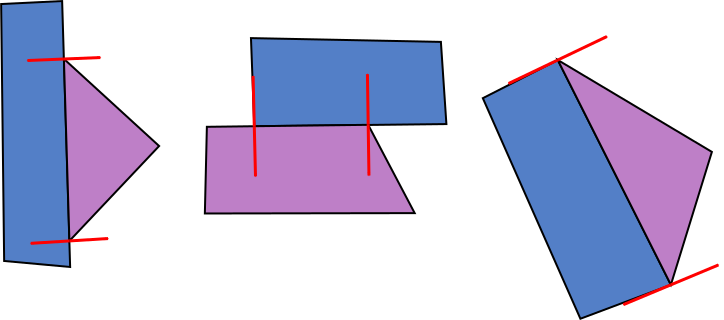
\includegraphics[width=0.75\textwidth]{images/cont_e2e}
\par\end{centering}
\caption{Edge-to-Edge contact examples.}
\end{figure}
\item [{\textbf{Vertex-Vertex}Vertex}] to inner vertex (in concave polygon)
is another type of discrete contact with multiple point-normal parameters.
Polygon 1 vertex is in contact with 2 edges of$p_{2}$. In this case,
since the movement of polygon 1 relative to polygon 2 is restricted
in 2 directions, 2 normal directions exist at same contact point.
The set of contacts for this variant consists of two contacts:$C=\{c_{1},c_{2}\},\;c_{i}=\left\{ r,\hat{n_{i}}\right\} $,
where$r$ stands for contact location and$\hat{n}$ stands for edges'
normal directions.
\begin{figure}[tbh]
\noindent \begin{centering}
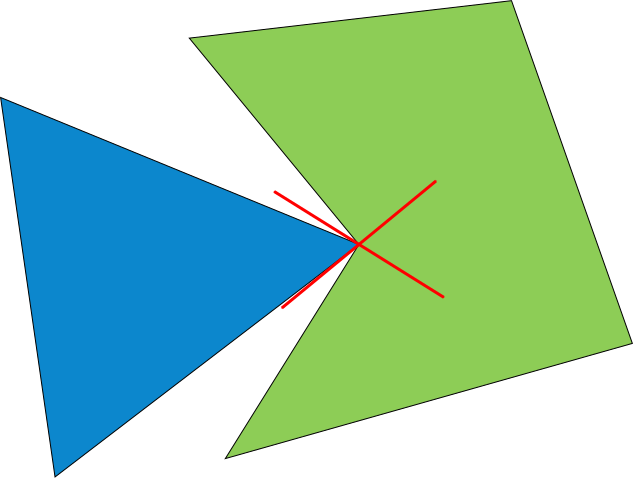
\includegraphics[width=0.35\textwidth]{images/cont_v2iv}
\par\end{centering}
\caption{Vertex-to-Inner-Vertex contact example.}
\end{figure}
\end{labeling}
Other variants of contact descriptions are variations of the mentioned
above. Examples: edge and inner vertex, vertex and vertex, edge and
edge. Outer vertex to outer vertex contact assumed to be unstable
and is discarded in this work. One polygon can contact several others
in distinct points, apart from a case where several vertices are coincident
as shown in\ref{fig:Multi-object-vertex}, in this case,
\begin{figure}[tbh]
\noindent \begin{centering}
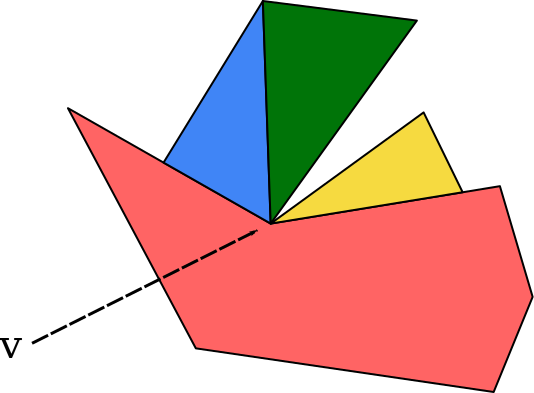
\includegraphics[width=0.45\textwidth]{images/multi-object-vertex}
\par\end{centering}
\caption{Multi-object vertex$v$.\label{fig:Multi-object-vertex}}
\end{figure}


\subsection{Contact description}

For the purpose of polygon arrangement evaluation, every contact is
assumed to be performed by polygon A acting on the polygon B. The
following description of a contact is adapted:
\begin{equation}
C=\left\{ id\left(P_{A}\right),id\left(P_{B}\right),p,\hat{n}\right\} 
\end{equation}
where$id\left(P\right)$ stands for polygon number/identification
entry,$p$ is a contact point location and$\hat{n}$ is the contact
normal direction inward the polygon B. An example of inter-object
contact description shown on\ref{fig:Contact-desription-example.}.
The contact is saved as:$C=\left\{ A,B,p,\hat{n}\right\} ,$where$A,B$
are the names of the polygons,$p$ is the contact location vector
in selected coordinate frame and$\hat{n}$ is the inward normal direction
of the second polygon at the contact location.
\begin{figure}[tbh]
\noindent \begin{centering}
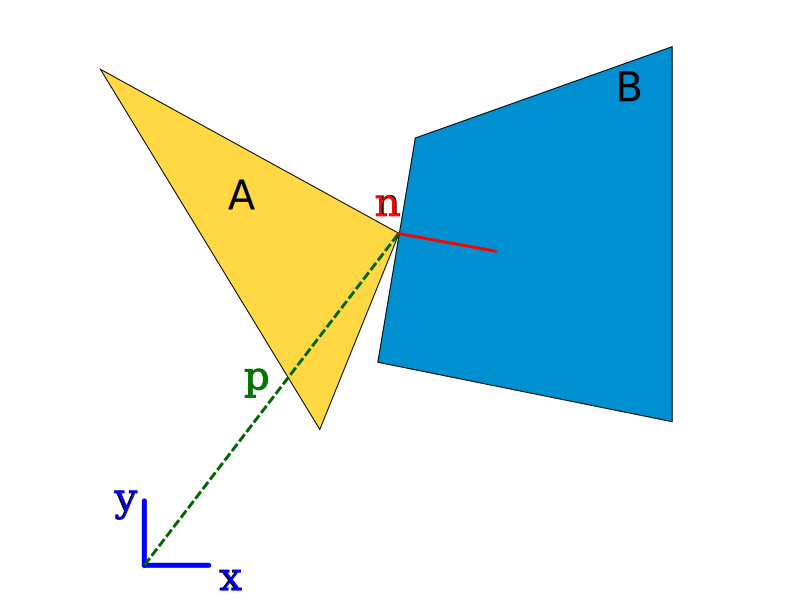
\includegraphics[width=0.55\textwidth]{images/cont_description}
\par\end{centering}
\caption{Contact description example.\label{fig:Contact-desription-example.}}
\end{figure}


\subsection{Solution existence for combination of internal and external contacts}

Given a set of polygonal objects, where some of the objects are in
contact one with another. Each object has at least 4 contacts: some
of them are fingers and some are inter-body contacts. The equilibrium
equation for each object is written in form of total wrench:
\begin{equation}
G\bar{f}=0
\end{equation}
where:$\bar{f}=\left[\begin{array}{cccccc}
f_{f1} & f_{f2} & f_{p12} & f_{p13} & \dots & f_{pMN}\end{array}\right]^{T}$ is a set of forces between fingers and bodies, and between bodies
and other bodies in contact.$G$ matrix rows multiplied by the set
of forces produce equations for$\begin{bmatrix}f_{x}\\
f_{y}\\
\tau
\end{bmatrix}=\begin{bmatrix}0\\
0\\
0
\end{bmatrix}$ for each body. The matrix will be block diagonal with some cross-block
columns which correspond to body-to-body contacts.
\begin{lem}
Given an edge of a polygonal object and a frictionless point contact,
the generalized (superposition) wrench for all possible locations
of contact along the edge can be expressed as 2 dimensional cone (2
vectors) in vertical plane of the configuration space (the plane's
normal direction will be in$f_{x}f_{y}$ plane).\label{lem:EGW-vertical}
\end{lem}
\begin{proof}
All possible contacts on the edge will have the same direction and
hence same$f_{x},f_{y}$ components. But for all these possible contacts
the wrenches will be different. The positions of the contact points
one the edge have limits, and at those limits will define the marginal
moments that the contact can apply. These two marginal vectors will
form a two dimensional cone in a wrench space.
\end{proof}
\begin{prop}
4 point fingers acting on a 2D object in distinct points along object's
boundary may constitute a force closure equilibrium grasp.
\end{prop}
\begin{proof}
Caratheodory's theorem shows that a N-dimensional space can be positively
span by N+1 vectors. For two-dimensional task space, there are 3 degrees
of freedom$\left(x,y,\theta\right)$ and hence both the configuration
space and the wrench space are three dimensional ($\rthree$). Four
distinct contacts can be represented be 4 vectors in the wrench space
and span it. Because of the configuration/wrench space duality, fully
spanned wrench space means fully constricted configuration space:
the object will have no freedom of movement. The convex hull of these
vectors spans the origin as well, and thus it is an equilibrium grasp.
\end{proof}
\begin{prop}
A set of$N$ polygonal objects in$\mathbb{R}^{2}$ in stable ( what
is stable contact ???) contact one with another can be immobilized
by at most$3N$ fingers assuming first order non-frictional contacts.\label{prop:3N_fingers}
\end{prop}
\begin{proof}
Given connected set of objects, for each object at least one contact
exist. For an object in$\mathbb{R}^{2}$ to be first order immobilized
minimum 4 constraints required. Knowing that at least one constraint
already exists because the set is connected, for each object 3 external
constrains are needed, yielding$3N$ fingers for the whole set.
\end{proof}
\begin{prop}
A set of$N$ polygonal objects in$\mathbb{R}^{2}$ in contact one
with another can be immobilized by at least 4 fingers assuming first
order contacts and exceptional resulting shape.
\end{prop}
\begin{proof}
Assuming optimal configuration of the objects where each of them is
immobilized relative to others by form closure conditions and possibly
external constraints ($EC$) the total amount of external constraints
for the set immobilization is$\max\left(4,\left|EC\right|\right)$.
Example: jigsaw puzzle which once assembled can be immobilized by
4 fingers.
\end{proof}
\begin{figure}[tbh]
\noindent \begin{centering}
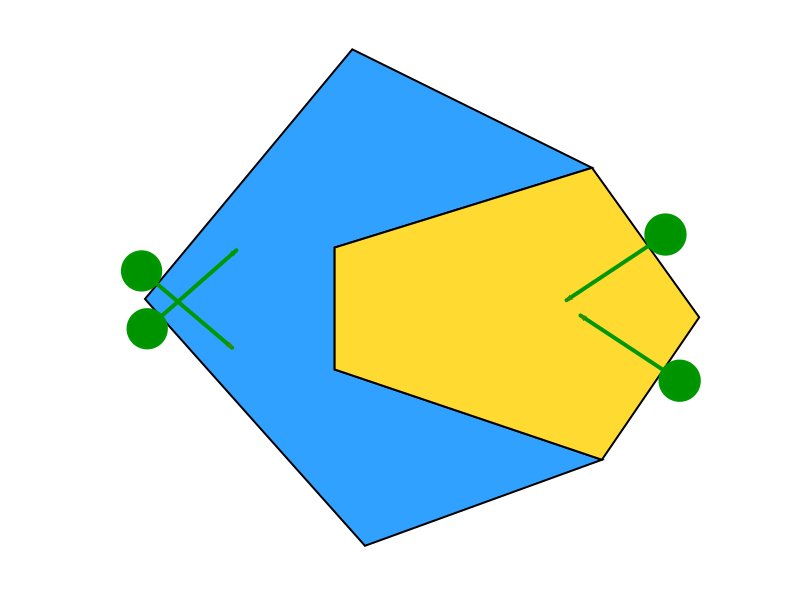
\includegraphics[width=0.45\textwidth]{images/minimum_4_fing}
\par\end{centering}
\caption{Immobilization by minimum 4 fingers.}
\end{figure}

\begin{prop}
Given a polygonal object and 3 parallel frictionless contacts on the
object boundary (same edge or different edges). It is impossible to
construct and first order immobilizing grasp with 1 additional contact.
\end{prop}
\begin{proof}
4 contacts of a frictionless grasp have to not to intersect in one
point, as showed\citet{Nguyen1986}. 3 parallel contacts are``intersecting''
at infinity. Moreover, 4-th contact alone cannot span all moments
around that intersection point.
\end{proof}
\begin{example}
\begin{figure}[tbh]
\noindent \begin{centering}
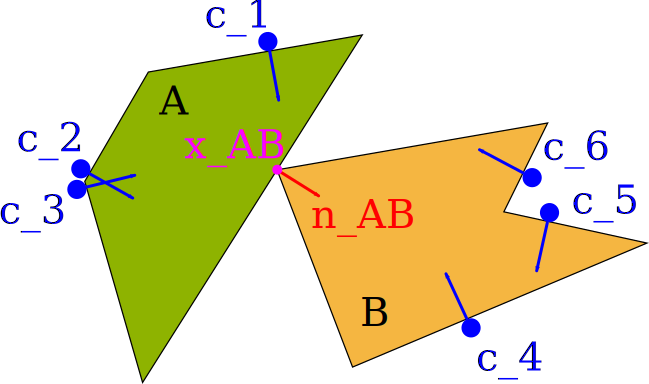
\includegraphics[width=0.55\textwidth]{images/solutions_existence}
\par\end{centering}
\caption{Solution existence example.}
\end{figure}
Two bodies in contact at one point. Contact forces shown in red, finger
forces shown in blue. Each force$f_{i}$ acts at point$\mathbf{x}_{i}$
located at body boundary, with direction$\theta_{i}$ which vector
is$\begin{bmatrix}\cos\theta_{i}\\
\sin\theta_{i}
\end{bmatrix}=\begin{bmatrix}c_{i}\\
s_{i}
\end{bmatrix}$. The inter-body contact force$f_{AB}$ selected to act in direction$\begin{bmatrix}c_{AB}\\
s_{AB}
\end{bmatrix}$ at point$\mathbf{x}_{AB}$. The objects are immobilized by 3 fingers,
according to the\ref{prop:3N_fingers}. Defining a grasp matrix for
fingers\emph{m} to\emph{n} (note the linear independence of the rows
in a matrix):
\begin{equation}
G_{f\left[m:n\right]}=\begin{bmatrix}c_{m} & ... & c_{n}\\
s_{m} & ... & s_{n}\\
\mathbf{x}_{m}\times\begin{bmatrix}c_{m}\\
s_{m}
\end{bmatrix} & ... & \mathbf{x}_{n}\times\begin{bmatrix}c_{n}\\
s_{n}
\end{bmatrix}
\end{bmatrix}
\end{equation}
such that in case of isolated 2D object
\begin{equation}
\begin{bmatrix}f_{Ax}\\
f_{Ay}\\
\tau_{A}
\end{bmatrix}=\begin{bmatrix}c_{1} & c_{2} & c_{3}\\
s_{1} & s_{2} & s_{3}\\
\mathbf{x}_{1}\times\begin{bmatrix}c_{1}\\
s_{1}
\end{bmatrix} & \mathbf{x}_{2}\times\begin{bmatrix}c_{2}\\
s_{2}
\end{bmatrix} & \mathbf{x}_{3}\times\begin{bmatrix}c_{3}\\
s_{3}
\end{bmatrix}
\end{bmatrix}\begin{bmatrix}f_{1}\\
f_{2}\\
f_{3}
\end{bmatrix}=G_{f\left[1:3\right]}\begin{bmatrix}f_{1}\\
f_{2}\\
f_{3}
\end{bmatrix}
\end{equation}
When there are 2 or more columns, 3rd row will only be a linear combination
of first 2 only if all contacts are in the same point:
\begin{equation}
G_{f\left[m,n\right]}=\begin{bmatrix}c_{m} & c_{n}\\
s_{m} & s_{n}\\
\mathbf{x}_{m}\times\begin{bmatrix}c_{m}\\
s_{m}
\end{bmatrix} & \mathbf{x}_{n}\times\begin{bmatrix}c_{n}\\
s_{n}
\end{bmatrix}
\end{bmatrix}=\begin{bmatrix}c_{m} & c_{n}\\
s_{m} & s_{n}\\
x_{m}s_{m}-y{}_{m}c_{m} & x_{n}s_{n}-y{}_{n}c_{n}
\end{bmatrix}
\end{equation}
\[
\rightarrow\mathbf{x}_{m}=\mathbf{x}_{n}
\]
Each$G_{f\left[m:n\right]}$ block consists of 3 rows and 1:3 columns.When
there is one column, third row is a linear combination of first 2:
\begin{equation}
G_{f\left[m\right]}=\begin{bmatrix}c_{m}\\
s_{m}\\
\mathbf{x}_{m}\times\begin{bmatrix}c_{m}\\
s_{m}
\end{bmatrix}
\end{bmatrix}=\begin{bmatrix}c_{m}\\
s_{m}\\
x_{m}s_{m}-y{}_{m}c_{m}
\end{bmatrix}
\end{equation}
In case of 1 finger contact on given body, 3rd row of the grasp matrix
(torque) will be linear combination of first 2 only if the finger
contacts is on the same locations as other (inter-body) contacts (and
has same direction), which by definition is neither feasible nor needed.
\end{example}
We can summarize the forces action on 2 bodies:

\begin{align}
\begin{bmatrix}f_{Ax}\\
f_{Ay}\\
\tau_{A}\\
f_{Bx}\\
f_{By}\\
\tau_{B}
\end{bmatrix} & =\left[\begin{array}{ccc}
G_{f\left[1:3\right]} & \left\{ \begin{array}{c}
-c_{AB}\\
-s_{AB}\\
-\mathbf{x}_{AB}\times\begin{bmatrix}c_{AB}\\
s_{AB}
\end{bmatrix}
\end{array}\right\}  & 0\\
0 & \left\{ \begin{array}{c}
c_{AB}\\
s_{AB}\\
\mathbf{x}_{AB}\times\begin{bmatrix}c_{AB}\\
s_{AB}
\end{bmatrix}
\end{array}\right\}  & G_{f\left[4:6\right]}
\end{array}\right]\begin{bmatrix}f_{1}\\
f_{2}\\
f_{3}\\
f_{AB}\\
f_{4}\\
f_{5}\\
f_{6}
\end{bmatrix}=\nonumber \\
= & \begin{bmatrix}G_{f\left[1:3\right]} & 0 & \left\{ \begin{array}{c}
-c_{AB}\\
-s_{AB}\\
\mathbf{-x}_{AB}\times\begin{bmatrix}c_{AB}\\
s_{AB}
\end{bmatrix}
\end{array}\right\} \\
0 & G_{f\left[4:6\right]} & \left\{ \begin{array}{c}
c_{AB}\\
s_{AB}\\
\mathbf{x}_{AB}\times\begin{bmatrix}c_{AB}\\
s_{AB}
\end{bmatrix}
\end{array}\right\} 
\end{bmatrix}\begin{bmatrix}f_{1}\\
f_{2}\\
f_{3}\\
f_{4}\\
f_{5}\\
f_{6}\\
f_{AB}
\end{bmatrix}=0\label{eq:Full-GM}
\end{align}
As seen in the\ref{eq:Full-GM} above, the grasp matrix for the given
set of objects consists of a diagonal blocks and off diagonal columns.
A system will be in equilibrium if a non-trivial set of forces exist
that solves the equation.

\z{Check the following, what is this? Do I need it at all? }

\emph{}

\subsection{Edge generalized wrench}

The evaluation of possible contact positions on an edged can be simplified
by introducing an edge generalized wrench:
\begin{figure}[tbh]
\noindent \begin{centering}
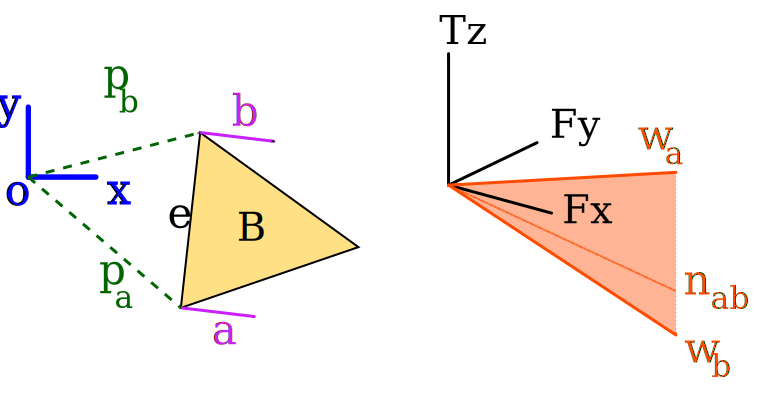
\includegraphics[width=0.75\textwidth]{images/Edge-Generalized-Wrench}
\par\end{centering}
\caption{EGW.}
\end{figure}

\begin{defn}
Given a polygon's edge\emph{e} and a reference point\emph{o,} the
set of all possible wrenches$w_{e}$ can can be defined by a two-dimensional
convex cone in a vertical plane of a wrench space.

Denote the edge's normal by$\hat{n}$ and edge's ends by$\vec{e}_{1},\vec{e}_{2}$
relative to\emph{o}, the edge is parameterized by parameter$s\in[0,1]$
the wrench of a contact along the edge can vary between:
\begin{equation}
\left(1-s\right)\begin{bmatrix}\hat{n}\\
\vec{e}_{1}\times\hat{n}
\end{bmatrix}+s\begin{bmatrix}\hat{n}\\
\vec{e}_{2}\times\hat{n}
\end{bmatrix},\qquad s\in[0,1]\label{eq:Edge-GW-parameterization}
\end{equation}
which is exactly a linear combination of two marginal wrenches. In
a geometrical representation, it is a planar angle contained in a
vertical plane (plane's normal direction has no torsional component)
in the wrench space. Illustration shows an example of a generalized
edge wrench. An edge of polygonal object B has inward normal direction$n_{ab}$.
Two marginal contacts$a,b$ are shown in violet, with locations defined
by vectors$p_{a},p_{b}$ respectively. Wrenches induced by these contacts
are calculated by:
\[
w_{a}=\begin{bmatrix}\hat{n}_{a}\\
\vec{p}_{a}\times\hat{n}_{a}
\end{bmatrix},\;w_{b}=\begin{bmatrix}\hat{n}_{b}\\
\vec{p}_{b}\times\hat{n}_{b}
\end{bmatrix}.
\]
As can be seen from the FIGURE , contact$a$ induces positive torque
about the selected reference point, while contact$b$ induces negative
torque. Hence, the 3-rd components of a wrench have opposite signs
and are located on different sides of the\emph{xy}-plane. The expression
for the edge generalized wrench can be rewritten to a form of:
\begin{align}
w_{e}\left(s\right) & =\left(1-s\right)\begin{bmatrix}\hat{n}\\
\vec{e}_{1}\times\hat{n}
\end{bmatrix}+s\begin{bmatrix}\hat{n}\\
\vec{e}_{2}\times\hat{n}
\end{bmatrix}=\begin{bmatrix}\hat{n}\\
\left(\left(1-s\right)\cdot\vec{e}_{1}+s\cdot\vec{e}_{2}\right)\times\hat{n}
\end{bmatrix},\qquad s\in[0,1]\nonumber \\
 & =\left[\begin{array}{c}
n_{x}\\
n_{y}\\
\left(x_{1}\cdot n_{y}-y_{1}\cdot n_{x}\right)+s\left(n_{y}\left(x_{2}-x_{1}\right)+n_{x}\left(y_{1}-y_{2}\right)\right)
\end{array}\right]\label{eq:EGW-parameterization}
\end{align}
We can note that only the torque component of the wrench vector changes
along the edge, and hence the edge generalized wrench is strictly``vertical''
in the wrench space, and that it is linear along the parameter\emph{s}.
\end{defn}

\subsection{Inverted cone test\label{subsec:Inverted-cone-test}}

As stated above, a convex hull of the contact wrenches should contain
the origin of a wrench space. Given several contacts, and corresponding
wrenches in the wrench space that do not contain the origin, a simple
test can show whether additional vector will make total convex hull
to contain the origin or not.
\begin{figure}[tbh]
\noindent \begin{centering}
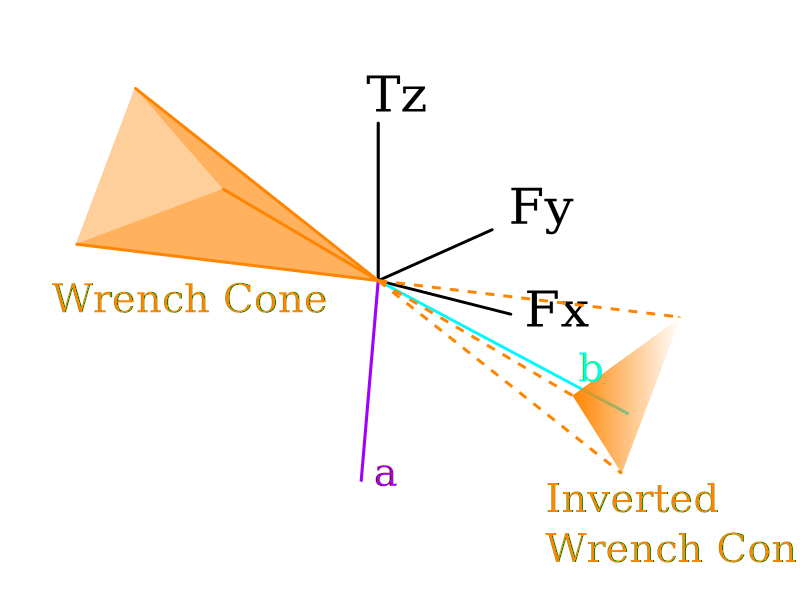
\includegraphics[width=0.75\textwidth]{images/inverted_cone_A}
\par\end{centering}
\caption{Inverted Cone, with vector\emph{$a$} inside and vector\emph{$b$}
outside.\label{fig:inv_cone_001}}
\end{figure}

\begin{prop}
Given a set of 3 contacts, whose wrenches do not span the wrench space
(the origin of the wrench space is not inside the convex hull of these
wrenches) while not being in the same plane and additional contact,
the contact can complete the force closure grasp of the object if
the contact's wrench lies within the inverted cone of the given contacts'
wrenches.\label{prop:InvCone-interior}
\end{prop}
\begin{proof}
Each couple of wrenches along with the origin point form a plane,
Equilibrium condition for a grasp is that the total wrench for all
contacts equals to zero:
\begin{equation}
\sum_{i=1}^{4}G_{i}f_{i}=0\label{eq:Total-Wrench}
\end{equation}
Where$G_{i}$ is$\begin{bmatrix}n_{i}\\
p_{c_{i}}\times n_{i}
\end{bmatrix}$\nomenclature{$n_{i}$}{i's contact inward normal direction \nomunit{[unitless]}}\nomenclature{$p_{c_{i}}$}{i's contact location in object's frame  \nomunit{[m]}}
for each contact. Rewriting the\ref{eq:Total-Wrench}:

\begin{equation}
G_{4}f_{4}=-\sum_{i=1}^{3}G_{i}f_{i}
\end{equation}
Given the fact that$G$ columns are wrench space vectors, and$f$
are scalar values, this allows the representation of a 4th wrench
space vector as a linear combination of other wrench vectors, which
is exactly the cone formed by these wrenches. If the 4th vector lies
outside the cone then it cannot be represented as a linear combination
of other wrenches and hence will not allow equilibrium grasp.
\end{proof}
\begin{example}
\label{exa::-A-square}A square object with 3 contacts
\begin{figure}[tbh]
\noindent \begin{centering}
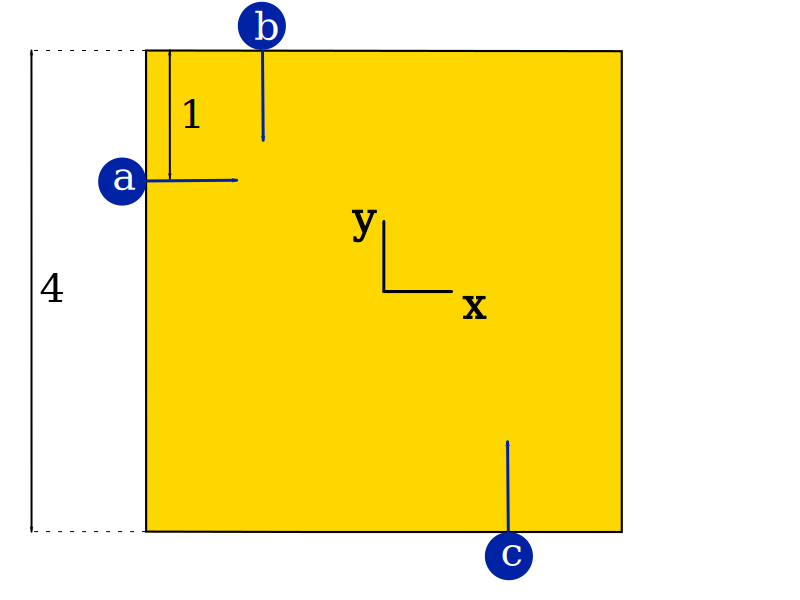
\includegraphics[width=0.45\textwidth]{images/example_inverted_cone_placement}
\par\end{centering}
\caption{A square object with 3 contacts.\label{fig:inv_cone_002}}
\end{figure}
. Each contact is located 1 unit length from an edge. The contacts
are described by the direction and the position as follows:
\[
C_{a}=\left\{ n_{a}=\begin{bmatrix}1\\
0
\end{bmatrix},p_{a}=\begin{bmatrix}-2\\
1
\end{bmatrix}\right\} 
\]
\[
C_{b}=\left\{ n_{b}=\begin{bmatrix}0\\
-1
\end{bmatrix},p_{b}=\begin{bmatrix}-1\\
2
\end{bmatrix}\right\} 
\]
\[
C_{c}=\left\{ n_{c}=\begin{bmatrix}0\\
1
\end{bmatrix},p_{c}=\begin{bmatrix}1\\
-2
\end{bmatrix}\right\} 
\]
Corresponding wrenches are:
\[
w_{a}=\begin{bmatrix}\hat{n}_{a}\\
\vec{p}_{a}\times\hat{n}_{a}
\end{bmatrix}=\begin{bmatrix}1\\
0\\
\begin{bmatrix}-2\\
1
\end{bmatrix}\times\begin{bmatrix}1\\
0
\end{bmatrix}
\end{bmatrix}=\begin{bmatrix}1\\
0\\
-1
\end{bmatrix}
\]
\[
w_{b}=\begin{bmatrix}\hat{n}_{b}\\
\vec{p}_{b}\times\hat{n}_{b}
\end{bmatrix}=\begin{bmatrix}0\\
-1\\
1
\end{bmatrix}
\]
\[
w_{c}=\begin{bmatrix}\hat{n}_{c}\\
\vec{p}_{c}\times\hat{n}_{c}
\end{bmatrix}=\begin{bmatrix}0\\
1\\
1
\end{bmatrix}
\]
Convex cone of these wrenches along with it's inverse are shown in\ref{fig:inv_cone_003}.
\begin{figure}[tbh]
\noindent \begin{centering}
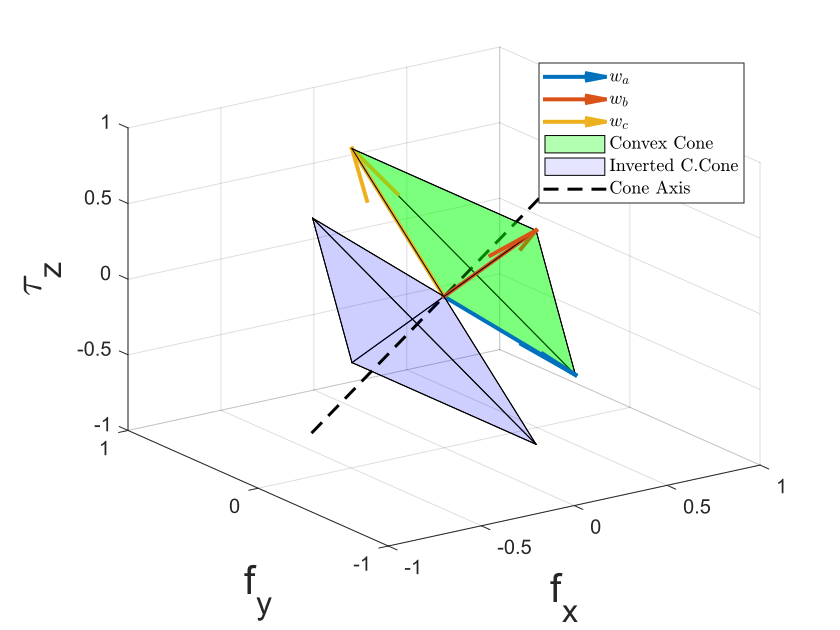
\includegraphics[width=0.75\textwidth]{images/example_inv_cone_01}
\par\end{centering}
\caption{Contact wrenches, convex cone and inverted convex cone.\label{fig:inv_cone_003}}
\end{figure}
The distance of some point from 3 faces of the inverted cone is calculated
by projecting the point onto the face normal. Face normal directions
are:
\[
\hat{n}_{ab}=\frac{w_{a}\times w_{b}}{\left|w_{a}\times w_{b}\right|}=\frac{\begin{bmatrix}1\\
0\\
-1
\end{bmatrix}\times\begin{bmatrix}0\\
-1\\
1
\end{bmatrix}}{\left|\begin{bmatrix}1\\
0\\
-1
\end{bmatrix}\times\begin{bmatrix}0\\
-1\\
1
\end{bmatrix}\right|}=-\frac{\sqrt{3}}{3}\left[\begin{array}{c}
1\\
1\\
1
\end{array}\right]
\]
\[
\hat{n}_{bc}=\frac{w_{b}\times w_{c}}{\left|w_{b}\times w_{c}\right|}=\frac{\begin{bmatrix}0\\
-1\\
1
\end{bmatrix}\times\begin{bmatrix}0\\
1\\
1
\end{bmatrix}}{\left|\begin{bmatrix}0\\
-1\\
1
\end{bmatrix}\times\begin{bmatrix}0\\
1\\
1
\end{bmatrix}\right|}=\begin{bmatrix}-1\\
0\\
0
\end{bmatrix}
\]
\[
\hat{n}_{ca}=\frac{w_{c}\times w_{a}}{\left|w_{c}\times w_{a}\right|}=\frac{\begin{bmatrix}0\\
1\\
1
\end{bmatrix}\times\begin{bmatrix}1\\
0\\
-1
\end{bmatrix}}{\left|\begin{bmatrix}0\\
1\\
1
\end{bmatrix}\times\begin{bmatrix}1\\
0\\
-1
\end{bmatrix}\right|}=\frac{\sqrt{3}}{3}\left[\begin{array}{c}
-1\\
1\\
-1
\end{array}\right]
\]
 Building generalized edge wrenches for each edge:
\begin{figure}[tbh]
\noindent \begin{centering}
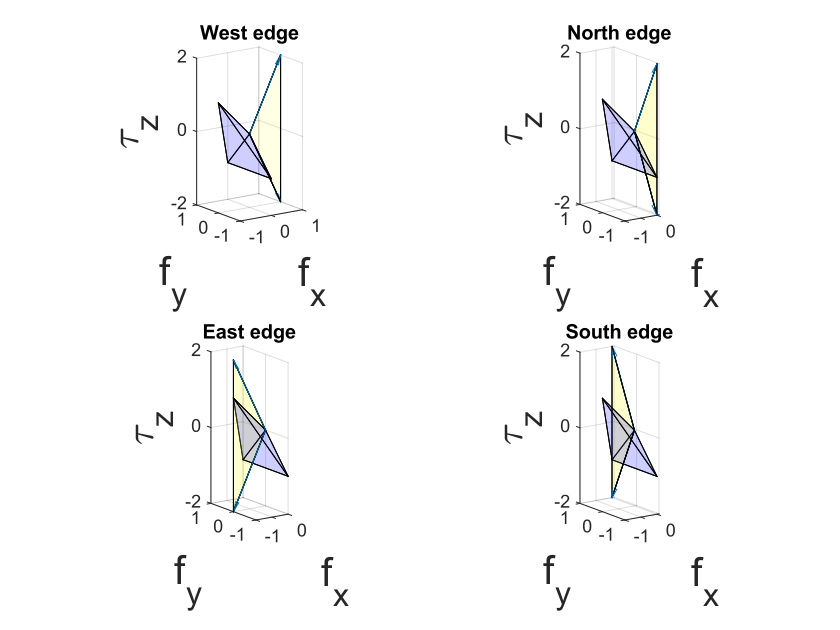
\includegraphics[width=0.75\textwidth]{images/example_inv_cone_02}
\par\end{centering}
\caption{Edge Generalized wrenches for 4 edges of the object.\label{fig:Edge-Generalized-wrenches}}
\end{figure}
As can be seen from\ref{fig:Edge-Generalized-wrenches}, only the
eastern edge wrench has the common intersection with the inverted
cone. Visual examination of the object confirms intuitively that placement
of a finger on the eastern edge only could immobilized the object.
It can be seen that only a wrench vector from the eastern edge can
complete the convex cone of 3 given contacts' wrenches and form a
convex hull which contains the origin in it's interior. Further development
shown in\ref{sec:Algorithms-for-finger}.
\end{example}

\subsection{Maximizing the Inscribed Sphere}

One of the proposed quality measures is a volume/radius of the sphere
inscribed in the convex hull of grasp map basis vectors. Maximizing
the sphere radius can be done by increasing the minimal of the distances
between the origin end the faces of the convex hull. Since the hull
is convex, some of the faces will be tangent to the sphere, and in
no case a edge will be tangent. In cases where several contacts act
on the object, it is always possible to construct a\emph{convex} hull
and thus eliminate redundant wrench vectors.
\begin{prop}
Given a set of k-1 contacts, and their corresponding wrench vectors,
convex cone and it's inverse cone; for a generalized wrench that has
a segment in the interior of the inverse convex cone an optimal k-th
contact can be found by examining distances of the convex hull faces
from the origin.
\end{prop}
\begin{proof}
As seen in\ref{prop:InvCone-interior}, the$w_{k}$ has to lie inside
of the Anti-Cone. If$w_{k}$ lies on a cone boundary then it and 2
vectors that form that boundary (denoted by$w_{1},w_{2}$), will form
a surface that contains the origin of the wrench space. To maximize
the distance of said surface from the origin we first parameterize
the wrench vector end point location segment by using the\ref{eq:EGW-parameterization}.
For each face of the convex hull, the distance of the face from the
origin can be calculated by projecting a point on the plane on the
plane's normal. We define a\emph{central axis} of their convex cone
as:
\[
a=\frac{\sum_{i=1}^{k-1}w_{i}}{\left|\sum_{i=1}^{k-1}w_{i}\right|}
\]
Assuming that the\emph{k-1} wrenches are sorted in counter-clock-wise
direction about the cone axis, meaning that
\[
a\cdot\left(w_{i}\times w_{i+1}\right)>0\;\forall i\in\left[1:k-1\right],
\]
\[
a\cdot\left(w_{k-1}\times w_{1}\right)>0.
\]
The equation for the normal direction of a plane formed by$w_{i},w_{i+1},w_{k}$
is:
\[
n_{p}=\left(w_{i}-w_{k}\right)\x{}\left(w_{i+1}-w_{k}\right).
\]
If the$w_{k}$ lies inside the inverted convex cone of first\emph{k-1}
contacts, then the normal direction will point from the plane towards
the origin. Consequently, the distance of the plane from the origin
can be expressed as:
\[
d_{i}=-w_{k}\cdot\left(w_{i}-w_{k}\right)\x{}\left(w_{i+1}-w_{k}\right),
\]
note the``-'' sign to obtain positive distance\footnote{MATLAB has polyshapes stored with vertices in clockwise direction,
hence no minus sign in the code.}. Substituting the expression for wrench vectors (shown in Appendix)
leaves the distance of plane\emph{i} (contacts\emph{i,i+1} and parameter\emph{s}along
an edge) to be a function of that parameter only:
\[
d_{i}=f\left(s\right),
\]
Ultimately, distance from every face can be expressed as a function
of edge parameter\emph{s} and thus a compound function of minimal
distance can be built.
\[
d=\min\left\{ d_{i}\right\} \;i\in\left[1,\right].
\]
Since projection is a linear transformation, and EGW endpoints segment
being parameterized uniformly, the distance function will be linearly
dependent on on\emph{s} parameter. Meaning that the distance function
will be either constant or monotonically increasing/decreasing along
the change in\emph{s}. Solution can be found by examining\emph{k-1}
1st order polynomials and finding the maximized minimal value. Since
the functions are 1st order polynomials, there either will be 1 such
solution or infinite number of solutions (in case where there is a
plane parallel to the EGW endpoints segment and hence the distance
is constant).
\end{proof}
\begin{figure}[tbh]
\noindent \centering{}\subfloat[Distance from convex cone faces.]{\noindent \begin{centering}
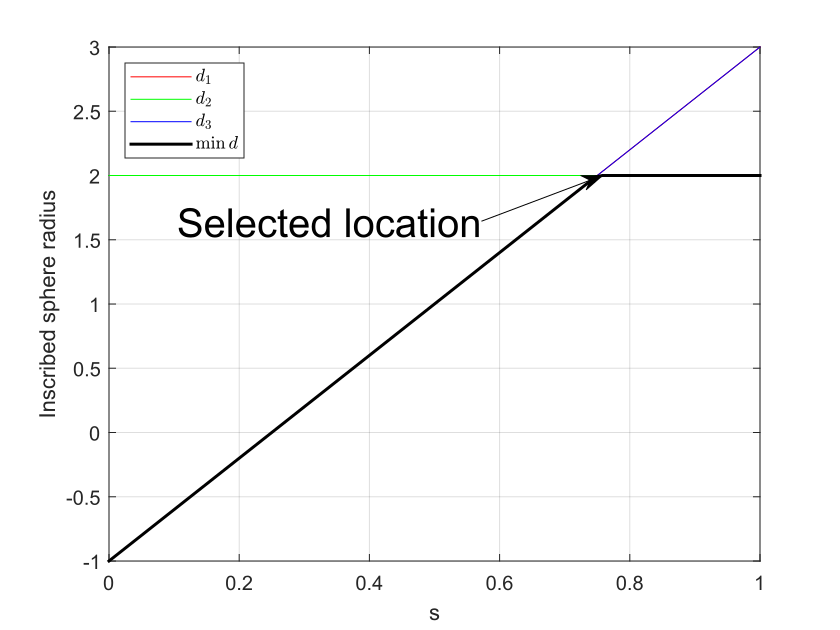
\includegraphics[width=0.45\columnwidth]{images/example_inv_cone_03}
\par\end{centering}
}\subfloat[Object with added contact]{\noindent \begin{centering}
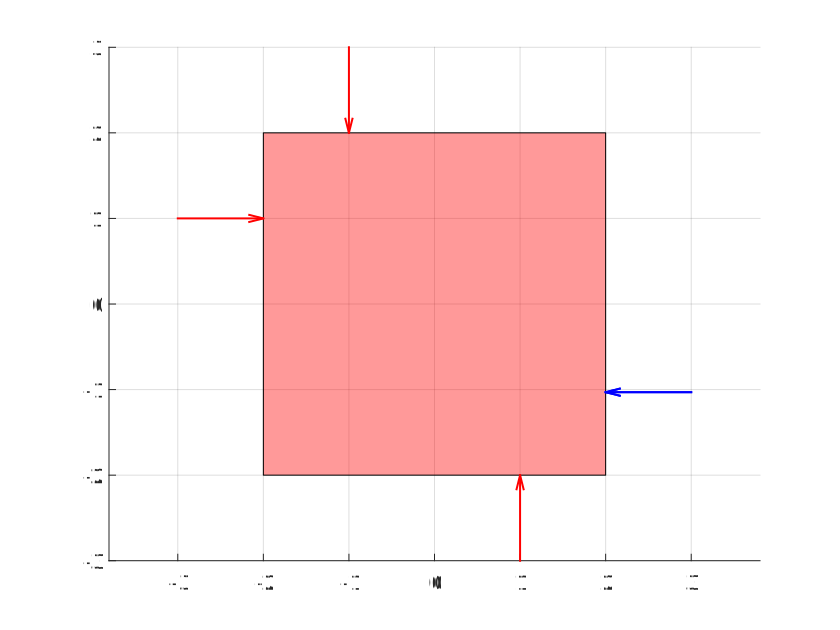
\includegraphics[width=0.45\columnwidth]{images/example_inv_cone_04}
\par\end{centering}
}\caption{Selecting the contact based on Inscribed Sphere Radius.\label{fig:Selecting-the-contact}}
\end{figure}
Elaborating on the\ref{exa::-A-square},\ref{fig:Selecting-the-contact}
presents distances from convex hull faces as function of the parameter\emph{s}.
In this case, due to the symmetry of the object and the contact locations,$d_{1}$
and$d_{3}$ are equal, while$d_{2}$ is constant. In this case one
of the distances is constant, and it is minimal at some part of the
domain. Contact point selected to be furthest from the brink. Additional
examples provided in Appendix.

\subsection{Connectivity graph search}

When a object arrangement is given (or obtained) and desired amount
of external constraints is found by proposed solution, there is no
guarantee that there is no sub-set of objects which is not immobilized.

This leads to a need of grasp assessment for sub-sets of the given
arrangement. Each connected sub-set should be tested and ensured to
be first order immobilized. Representing the objects arrangement as
a connected graph one can find all connected sub-graphs. Several methods
available for sub-graphs extractions based on different criteria,
such as\citet{Ullmann1976,Bron1973,Gouda2010} but for practical purposes
simple algorithm is used:

Recursively excluding nodes and checking whether connected graphs
exist. If so - add them to the connected sub-graphs list. This can
be implemented both as Depth First Search and as Breadth First Search.

\begin{figure}[tbh]
\noindent \begin{centering}
\subfloat[Full graph]{\noindent \begin{centering}
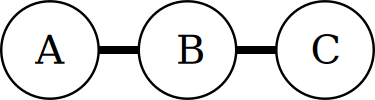
\includegraphics[width=0.3\columnwidth]{images/graph_example_a}
\par\end{centering}
}\subfloat[B node removed\protect \\
no connected subgraphs]{\noindent \begin{centering}
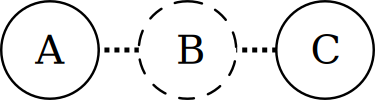
\includegraphics[width=0.3\columnwidth]{images/graph_example_b}
\par\end{centering}
}\subfloat[C node removed\protect \\
AB subgraph is connected]{\noindent \begin{centering}
\includegraphics[width=0.3\columnwidth]{images/graph_example_c}
\par\end{centering}
}
\par\end{centering}
\caption{Graph, connected and disconnected subgraphs}
\end{figure}


\subsection{Grasp quality measure for a set of objects}

Assessment of the Grasp Quality Measure can be performed for given
subset. Note that Grasp Quality Measure for single object and for
constellation of several object may have different trends at given
finger configuration: the grasp may be optimal for the object, but
for the constellation it will yield not the highest value.
\begin{example}
2 objects in contact. each object is immobilized individually, and
the whole constellation is immobilized as well. Examining the grasps
by computing GQMs shows that individual GQMs are high (maximal values)
but total GQM (due to external contact vectors only) is low due to
the directions of the external fingers contacts.

\ref{fig:GQMs-difference.} shows two polygonal objects immobilized
by 4 external contacts. External contact direction vectors have relatively
low\emph{y}-components, and hence limit the GQM inscribed sphere radius
to be at most as large as the\emph{y}-component of the wrench vectors.
The individual convex hulls are significantly larger the the convex
hull for the both objects together.
\end{example}
\begin{figure}[tbh]
\noindent \centering{}\subfloat[Immobilized objects.]{\noindent \begin{centering}
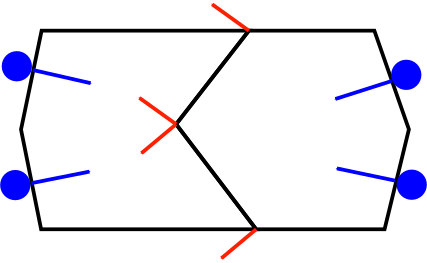
\includegraphics[width=0.35\textwidth]{images/GQMs}
\par\end{centering}
}\subfloat[Convex Hull for each object and for the set (red).]{\noindent \begin{centering}
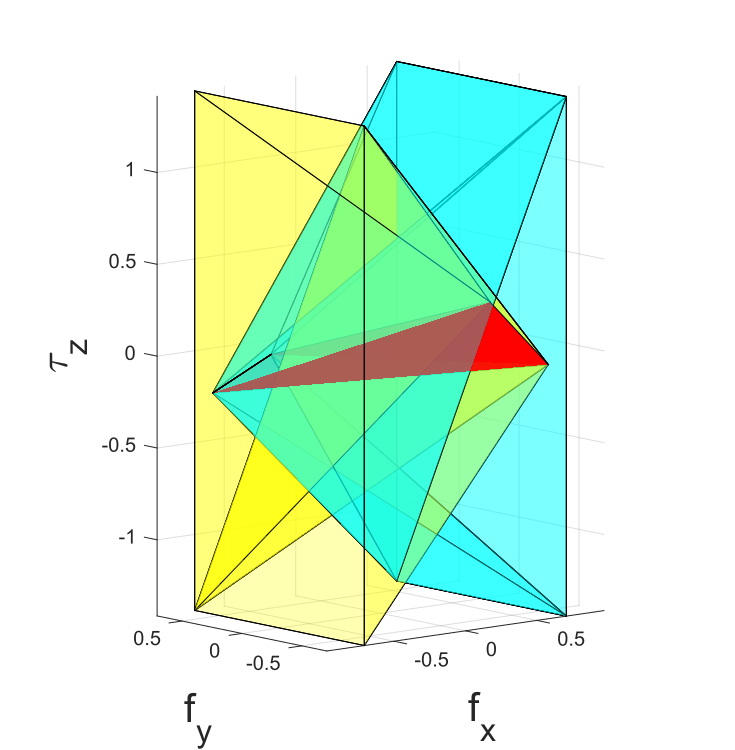
\includegraphics[width=0.35\textwidth]{images/GQM_set_vs_one}
\par\end{centering}
}\caption{GQMs differences.\label{fig:GQMs-difference.}}
\end{figure}


\section{Determining new configuration for objects}

\subsection{Description}

\subsection{Pseudocode}

Given an unordered set of objects, each object is scanned and classified:
number of edges, concave vertices, edges' lengths. Scanned and classified
objects allow assessment of different constellations for future grasping.
Based on the algorithms and inter-object contacts classification as
presented above, several strategies for object rearrangement can be
implemented.

The approach for objects rearrangement is to stack objects in configuration
that will require amount of minimal fingers for each object, maximizing
number of inter-object effective contacts. Objects in the set in the
new configuration can be described by a tree, where the root is some
selected object, and all other objects described as children in a
way similar to URDF style\citep{ros.org2009}.

First of all, we need to know how many polygons with concave vertices
exist, and how many exist with vertex angles less than $90\text{�}$.
Additionally, how many angles are smaller than concave angles if any.

Recapping the inter object contact types along with the additional
contacts needed for the immobilization, we assume that the parent
object is immobilized and inducing contact forces on a child object,
which has to be immobilized by additional fingers. In the following
paragraphs, term``fixation'' refers to the contacts of the parent
object acting on the child object.

\textbf{Edge-to-edge} fixation provides two parallel contacts, their
convex cone can be seen as infinite ``corridor'', formed by the
contact region swept along the contacts' normal direction. The interaction
can be considered useful in cases where some other 2 different edges
provide normal directions that are crossing in the parallel contacts'
``corridor''. Simple example would be a case with a vertex inside
of the ``corridor'', where normal directions of 2 adjacent edges
induce opposite wrenches about the edge with two contacts. This requires
at least 2 additional external contacts for each object to complete
the fixture.

One way of finding such configuration is checking whether there exists
an object with a vertex (concave or convex) that is projected on the
interior of some non-adjacent edge (base edge), the edge can be used
as a base of edge-to-edge contact, and the vertex's adjacent edges
will serve as locations for 2 additional fingers. The grasp will be
feasible if normal directions from the adjacent edges and from the
base edge will positively span $\rtwo$. Example of feasible and non
feasible grasps are shown in \ref{fig:Edge-infinite-projection}.
\begin{figure}[tbh]
\noindent \centering{}\subfloat[Spanning vectors]{\noindent \begin{centering}
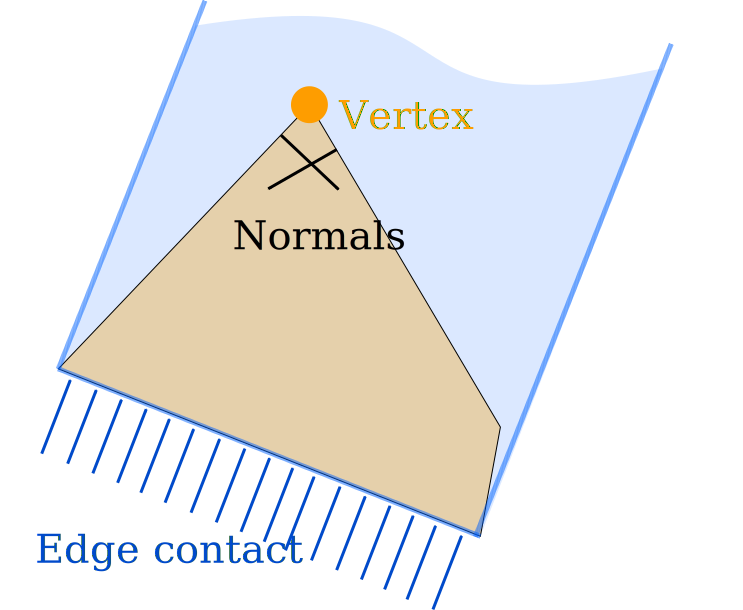
\includegraphics[width=0.35\textwidth]{images/OP_e2e}
\par\end{centering}
}\subfloat[Not spanning vectors]{\noindent \begin{centering}
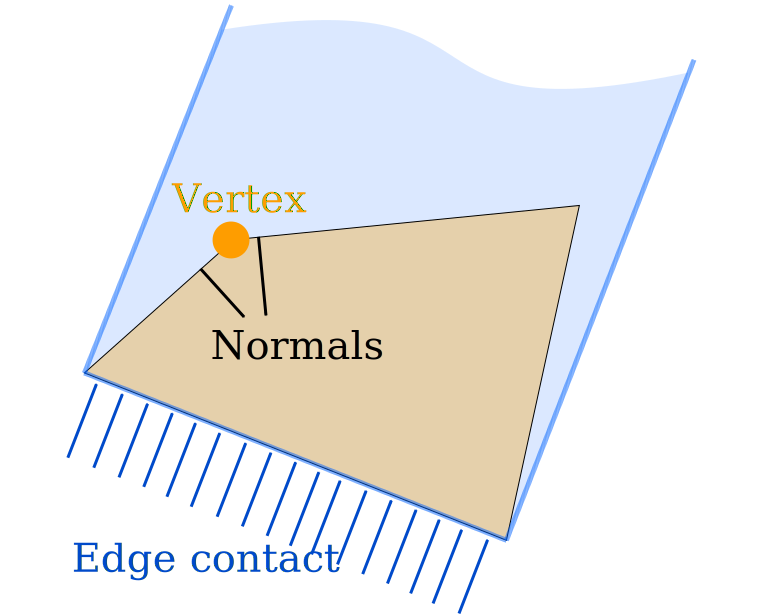
\includegraphics[width=0.35\textwidth]{images/OP_e2e_02}
\par\end{centering}
}\caption{Edge infinite projection and vertex with adjacent normal vectors.\label{fig:Edge-infinite-projection}}
\end{figure}

\textbf{Vertex-to-inner-vertex}fixation provides 2 edges normal directions,
which yield a convex cone with distinct vertex (unlike two parallel
contacts which can be considered as convex cone with a vertex at infinity).

This fixation allows use of single edge to complete the fixture, given
that the edge's inner normal direction is a negative combination of
the given contacts' directions, and the edge allows two distinct contacts
with opposing wrenches about the vertex (i.e. vertex is projected
on the inner of the edge segment), as shown in \figref{In-v-a}. In
case no such edge exist, two different edges provide normal directions
which form a convex cone that mutually overlap(have a common region)
the given convex cone (or their anti-cones), and the line connecting
the vertices of the cones is in the interior of the overlapping region.
\begin{figure}[tbh]
\noindent \begin{centering}
\subfloat[\label{fig:In-v-a}]{\noindent \begin{centering}
\includegraphics[width=0.35\textwidth]{images/OP_v2iv}
\par\end{centering}
}\subfloat[\label{fig:In-v-b}]{\noindent \begin{centering}
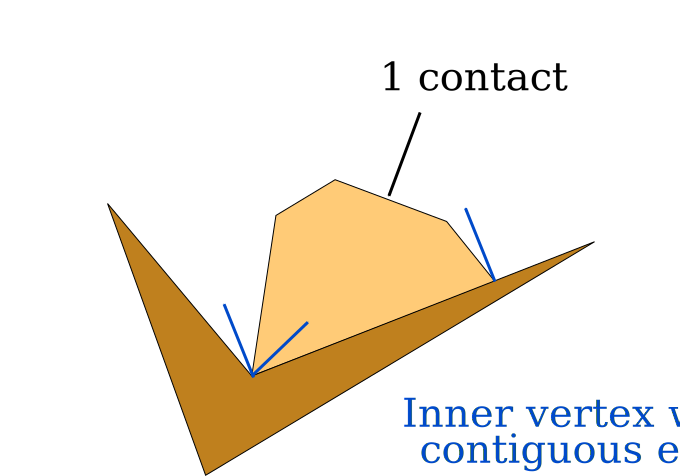
\includegraphics[width=0.35\textwidth]{images/OP_v2iv_ce}
\par\end{centering}
}
\par\end{centering}
\noindent \centering{}\caption{Inner vertex immobilization.\label{fig:Inner-vertex.}}
\end{figure}

\textbf{Vertex-to-inner-vertex with contiguous edge}fixation contributes
3 effective contacts and needs only one external finger contact in
the optimal case. For this there should exist an edge which projection
along it's normal direction has 2-contact vertex inside it's interior
and a there exists an intersecting segment of that projection and
the 3rd normal direction that lies inside the convex cone of first
2 normals. Example of such configuration is shown in \ref{fig:In-v-b}.
If no such edge exists, 2 external contacts are required to immobilize
this grasp by a method presented above

Vertex-to-inner-vertex with 2 contiguous edges fixation provides a
optimal configuration which requires sole external contact for the
immobilization of the object. Since objects are polygonal objects
with non intersection edges and non-zero thickness, there will always
exist an edge with a normal direction that will complete the form
closure.

Vertex-to-inner-vertex with a contiguous edge and a contact point
fixation is similar to the previous one except for the normal direction,
and hence in certain cases can be self immobilizing.

Vertex-to-inner-vertex with additional contact points are equivalent
to the vertex-to-inner-vertex with contiguous edges formations. The
provide same amount of contacts, but the normal directions can differ.

\textbf{Contiguous edge with vertex point contact} fixation forms
a case with 3 contacts, which allows fixation with one additional
finger under certain conditions: there should exist an edge, which
projections common segment with the point contact's normal has a part
lying inside the edge contact's infinite projection and also the new
edge, point and given edge normal directions should span $\rtwo$.\ref{fig:Contiguous-edge-with}
shows an example of possible contact locations for this fixation.

Example on \ref{fig:2-Contiguous-edges.} describes 2 contiguous edges,
which can be seen as sub case for the described fixation and any contact
with normal direction which is negative linear combination of the
normals of 2 edges will immobilize the object.
\begin{figure}[tbh]
\begin{centering}
\subfloat[Contiguous edge with point contact.\label{fig:Contiguous-edge-with}]{\noindent \begin{centering}
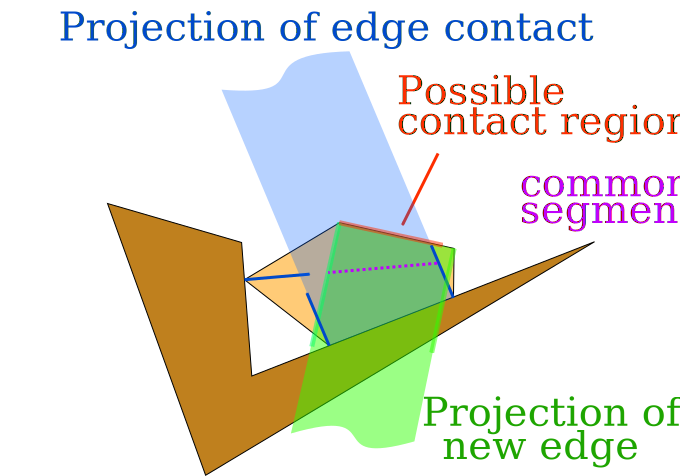
\includegraphics[width=0.35\textwidth]{images/OP_c2_p}
\par\end{centering}
}\subfloat[2 Contiguous edges.\label{fig:2-Contiguous-edges.}]{\noindent \begin{centering}
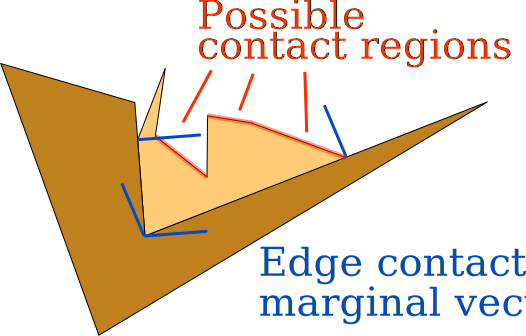
\includegraphics[width=0.35\textwidth]{images/OP_cc2}
\par\end{centering}
}
\par\end{centering}
\caption{Example of preferred edge contacts.}
\end{figure}

\LyXZeroWidthSpace Given all these considerations, presented set of
objects can be arranged to require the minimal amount of external
fingers for each object and hence minimal amount of fingers in total.

The order of the stacking is suitable for the one-by-one object manipulation.
Possible inter-object fixations can be ordered by amount and restrictions
on additional contacts that are to be applied.\ref{fig:Object-placement-priority.}
describes the order of preferable inter-object relations, based on
amount of external fingers needed for the immobilization of child
object relative to the parent.

\begin{figure}[H]
\begin{centering}
\begin{center}
\smartdiagramset{set color list={green,green,green,yellow,orange,red},
back arrow disabled=true}
\smartdiagram[descriptive diagram]{
  {1,{Vertex-to-inner-vertex\\ 2 contiguous edges}},
  {1,{Vertex-to-inner-vertex\\ 1 contiguous edge with point contact}},
  {1,{Vertex-to-inner-vertex\\ 1 contiguous edge}},
  {2, {Edge to edge}},
  {2, {Vertex-to-inner-vertex}},
  {2+, {Vertex to edge}},
}
\end{center}
\par\end{centering}
\caption{Object placement priority.\label{fig:Object-placement-priority.}}
\end{figure}

Basically, last option (vertex to edge) will never be selected intentionally
since if there is an option to place an vertex on an edge, there also
is an option to place edge on edge. Vertex-to-inner vertex option
also exists but for stability it is preferred to rotate the child
object so it will have more parent contacts - vertex-to-inner-vertex
with a contiguous edge.

First step is to define a root object, which will serve as base for
further object stacking. This is done either by selecting a polygon
with concave vertex, or stacking together two objects to form a concavity.

\begin{algorithm}[H]
\caption{Defining the root object}   
\KwData{Set of polygons $P = {p_i}\;i\in \left[ 1,K \right]$}
\KwResult{Tree of objects including the root object and possibly one child; defining the root concavity.}
\eIf{$\exists$ 1+ concave vertices}
{
	Root object = $p_i$ with widest concave vertex\;
}
{ % No concave vertices
	\eIf{$\exists$ 2 vertices with inner angles $\geq 90 \textdegree$}
	{
		Root = $p$ with greatest angle\;
		Root.Child(k) = $p$ with second greatest angle\;
		Align vertices to conctact, child leans on longest adjacent edge of the parent\;
	}
	{
		Root = $p$ with longest edge\;
		Root.Child(k) = $p$ with second longest edge\;
		Align longest edges to be collinear, vertex on child's longest edge coincident with midpoint of parent's longest edge.\;
	}
}
\end{algorithm}

When root object is determined, further stacking can be done. If there
are objects with vertex angles less than the concavity angle, they
are stacked together inside the concavity, possibly forming multiple
concavities. If no such object exists, an object that will form a
new concavity is stacked inside the root concavity.

\begin{algorithm}[H]
\caption{Objects stacking}   
\KwData{Set of polygons $P = {p_i}\;i\in \left[ 1,K \right]$, Object tree $T$}
\KwResult{Complete tree defining the configuration of the set of of objects.}
$C = \textrm{list of concavities}$\;
initialize C with the root concavity\;
L = $\left\{ v\right\}  $ sorted list of polygon vertices\; % with $\angle v \leq \angle \left( C \right)  $
\ForEach{$v \in L$}
{
	\eIf{$\angle \left( v \right) \leq \angle \left( c_i  \in C \right)$}
	{
		Stack the child object in the $c_i$, \emph{vertex to innter vertex}, edge aligned preferrably to a edge with non equal length\;
		$\textrm{move } L.v \textrm{ to } T.v $ and save child location and orientation\;
		$C.c_i = \textrm{reduced concavity}$\;
		$C = \textrm{new formed concavities}$\tcc*[r]{Upd. concavities list}
	}
	{
		Find smallest concavity that allows \emph{contiguous edge with vertex contact} interaction, stack object there.
		$C = \textrm{new formed concavities}$\;
	}
}
\end{algorithm}

\z{What if there are no concavities after several stacking steps?}

After the desired configuration is obtained, finger contact locations
can be obtained using the algorithms in \ref{sec:Algorithms-for-finger}.
The locations that are found should be tested to complete a form closure
grasp, 

\z{What about:\\
Description\\
Completeness\\
Complexity\\
}

\section{Contacts search}

Given a set of polygonal objects, first step is to find the contacts
between the objects. The problem is subdivided into assessment of
polygon pairs. The polygon interactions assessed by simple algorithm
that checks whether vertices of one polygon lie on edges or on vertices
of another one. Due to the complexity of the process, it is split
to 2 parts: specific point on polygon evaluation and contact search
for the polygons. \z{Add part where regions allowed for finger placement are saved as well.}

The algorithm \# detects whether a given point belongs to a boundary
of given polygon, whether along the edge or on one of the vertices.

\begin{algorithm}[H]
\caption{$\mathtt{p\_on\_Polygon}\qquad$}    % Determine whether a point is on polygon boundary
\KwData{Point $p$, polygon $P$}
\KwResult{Boolean True if the point lies on polygon boundary}

\For{$e_1,e_2$ = adjacent vertices of $P$}
	{
%\If{$\mathtt{p\_on\_e}\left(p,e_1,e_2\right)$}
\If{$p_i$ is on segment $e_{12}$}
			{\KwRet{True}\;}
	}
\KwRet{False}\;
\end{algorithm}

The algorithm \# is used to perform an inspection of contact points
for given 2 polygons. The algorithm finds contacts between 2 polygons,
returning a set that contains all contacts both the location and direction
of the contact and the polygons IDs (numbers) that the contact relates
to.

\begin{algorithm}[H]
\label{alg:C_from_2P}
\caption{$\mathtt{C\_from\_2P}\qquad$}    % Find contact points between 2 polygons
\KwData{Polygons $P_1$, $P_2$}
\KwResult{C: Set of contacts between 2 polygons}
	C $\longleftarrow\{\varnothing\}$\tcp*{Initialize empty contact set}
\For{$p_i$ = vertex of $P_1$}{
\If{$\mathtt{p\_on\_Polygon}\left(p_i,P_2\right)$}{
\eIf{$p_i$ is a vertex of  $P_2$}{
\uIf{$p_i$ is inner vertex of $P_2$}{
					$V_1$ = normal at $p_i$ to adjacent edge\#1 of $P_2$\;
					$V_2$ = normal at $p_i$ to adjacent edge\#2 of $P_2$\;
					C $\twoheadleftarrow\{id\left(P_1\right), id\left(P_2\right), p_i,V_1\}$\;
					C $\twoheadleftarrow\{id\left(P_1\right), id\left(P_2\right), p_i,V_2\}$\;
				}
\ElseIf{$p_i$ is inner vertex of $P_1$}{
					$V_1$ = normal at $p_i$ to adjacent edge\#1 of $P_1$\;
					$V_2$ = normal at $p_i$ to adjacent edge\#2 of $P_1$\;
					C $\twoheadleftarrow\{id\left(P_2\right), id\left(P_1\right), p_i,V_1\}$\;
					C $\twoheadleftarrow\{id\left(P_2\right), id\left(P_1\right), p_i,V_2\}$\;
				}
\tcc{append the contact to contact set TWICE, for each normal direction, along with with polygons' IDs}
			}
			{
				V = normal at $p_i$ to $P_2$\;
				C $\twoheadleftarrow\{id\left(P_1\right), id\left(P_2\right), p_i,V\}$\;
\tcc{append the contact to contact set, along with polygons' IDs}
			}
		}
	}
\For{$p_i$ = vertex of $P_2$}
	{
\If{$\mathtt{p\_on\_Polygon}\left(p_i,P_1\right)$\textrm{and} $p_i$ is not a vertex of $P_1$}
		{
				V = normal at $p_i$ to $P_1$\;
				C $\twoheadleftarrow\{id\left(P_1\right), id\left(P_2\right), p_i,V\}$\;
\tcc{append the contact to contact set, along with polygons' IDs}

		}
	}
\end{algorithm}

Once all contacts between all polygons are determined, remaining needed
fingers placement can be done for each polygon.

Given a polygon, and a set of contacts acting on that polygon, a remaining
amount of fingers needed can be determined.

The methods relies on a fact that 4 frictionless contacts is a minimum
for immobilization of a two dimensional object.

\section{Fingers placement\label{sec:Algorithms-for-finger}}

\subsection{Description}

Given a configuration of objects in contact (single group, each object
has at least one contact), the configuration is parameterized by contact
types. Each inter-object interaction is classified according to the
variants defined above in\ref{subsec:Relationship-between-polygons}.
When all contacts are found, each object is checked and an amount
of additional contacts for first order form closure is derived. For
every object all missing fingers are found.

Several methods for single object finger placement were developed
(presented in\ref{sec:Literature-Review}). For the purposes of this
work 2 (??) methods were compared: moment-labeling based contact point
derivation and grasp quality measure assessed random contact point
placement with constraints.

Next step is to perform a check, whether any group of objects is not
immobilized. A connectivity graph is build for given configuration.
Connected sub-graphs are extracted from the given graph, and corresponding
object constellations are tested for 1st order immobilization. If
the constellation is not immobilized (see examples \#ADDFIG) additional
fingers are placed while the constellation is treated like a single
object.

After all the variants are checked we can conclude that the group
of objects is immobilized.

Steps of the algorithm.\ref{alg:C_from_2P}

\z{What about masking the edges that are not available for grasp?
Formal description?
Flowchart}

The global finger placement process is divided to several cases of
polygon contact combinations. Cases of existing 3,2 and 1 inter-object
contacts are addressed. When possible, contact locations selected
to yield highest grasp quality measure, namely origin centered inscribed
sphere radius.

\subsection{Pseudocode}

\paragraph{Finding 1 finger contact given 3+ contacts on an object}

Given 3 contacts on an object, the viable regions for the 4th finger
can be determined by evaluating for each edge whether it is possible
to achieve a force closure grasp by placing a finger on that edge.
When existing contacts represented by wrench space vectors, it is
possible to perform assessment of the convex cone and convex hull.
For a convex hull of 4 wrenches to span the origin of the wrench space,
any 3 of the vectors should be linearly independent (not lying in
one plane) and the 4th vector should be a negative combination of
first 3, as shown in\ref{subsec:Inverted-cone-test}. If there exists
such wrench, corresponding contact location can be selected to be
a complementary finger contact. Since on every edge could exist variety
of possible contacts, simple quality measure presented in\ref{subsec:Inverted-cone-test}
is used to select the most promising contact location. The algorithm
is presented below:

\begin{algorithm}[H]
\label{alg:contact4}
\caption{$\mathtt{c4\_for\_P\_given\_3c}\qquad$}    % Determine the region for 4th contact given 3
\KwData{Polygon: $P$, 3 contacts: $C_i\,,\; i=1,2,3$}
\KwResult{$CP_4 =\{ p_i, GQM_i\}$: a set of locations for 4th contact to form desired grasp}

	$AntiCone =-1\cdot Cone\left(\{ w_{C_i}\},i=1,2,3\right)$\;
	$ConeAxis =-\sum_{i=1}^3 w_{C_i} $\;
\tcc{Form a cone of given contacts}

\For{$e_i$ = edge of $P$}
	{
		$GW = GeneralizedWrench(e_i)$\; %\tcp*{Create a generalized wrench for the edge}
\tcc{Create a generalized wrench for the edge}
		$CS = CommonSegment(GW, AntiCone)$\;
\tcc{Find a part of the generalized wrench that is inside of the Anti Cone}
\If{$CS\neq\varnothing$}
		{
\tcc{If there are wrenches that lie inside of Anti Cone determine the loci of possible contacts that will form a grasp}

			$w_{optimal} = Projection(ConeAxis, GW)$\;
			$GQM_i = GraspQualityMeasure\left(\left.w_{C_{k}}\right|_{k=1:3},w_{optimal}\right)$\;
\tcc{A vector that yields highest GRASP QUALITY MEASURE is the one that has highest projected length on the central axis of the AntiCone}
			$CP_4\twoheadleftarrow\{\mathtt{locationFromWrench}\left(w_{optimal}\right), GQM_i\}$\;
		}
	}
\end{algorithm}

The algorithms gives a solution for cases where 3 given contacts'
wrench space vectors are linearly independent. If one of the contacts
is a combination of other two - 2 marginal vectors that form the convex
cone that includes the 3rd one should be chosen and passed to algorithm$\mathtt{c3,c4\_for\_P\_given\_2c}$.
This method is complete and guaranteed to find a solution if there
exist one. The method is computationally inexpensive - O(n), it iterates
over the number of edges at most one time. NEED SOME IMAGE HERE \#ADDFIG

Set some error margins for placement uncertainty. \#CHECK again the
logic in this sections, see if it matches the one presented in the
class on July 29.

\z{Given 3 distinct contacts on a polygonal object a search is done whether it is possible to immobilize the object by one finger.\\
If 3 contacts are parallel or intersect at one point - it is impossible to form an immobilizing grasp by 1 additional finger as mentioned above (REF).\\
Assuming that 3 contacts are valid, the possible areas for placing a 4-th contact can be done in the following way:\\
Selecting two (non-parallel) contacts and form a cone along with anti-cone. Check whether a 3rd contact has a segment inside the cone or the anti-cone or both. Check whether that segment(s) has normal projections on edges of the polygon. For every edge that got a real projection of the segment on it form a }

\paragraph{Finding 1 finger contact for symmetric 4+ contacts}

In multi-object configurations, in particular in those that generated
for minimal finger grasping, cases with more than 4 contacts can act
on a given object. In such cases possible position of one or more
additional fingers can be determined in a way similar to the algorithm
presented above.

Given inter-object contacts will form a convex cone of wrench vectors.
Each edge can be tested to have a segment of generalized edge wrench
inside of the anti-cone of given contacts. If such segment exists,
optimal finger placement location can be selected and saved along
with the region allowed for finger placement. If given contacts yield
a zero-volume convex cone - 2 fingers are tested to complete grasp
according to the algorithm \#.

Example:\ref{fig:4-contacts} shows 2 bodies in contact, 4 distinct
contact forces act on each body.
\begin{figure}[tbh]
\noindent \begin{centering}
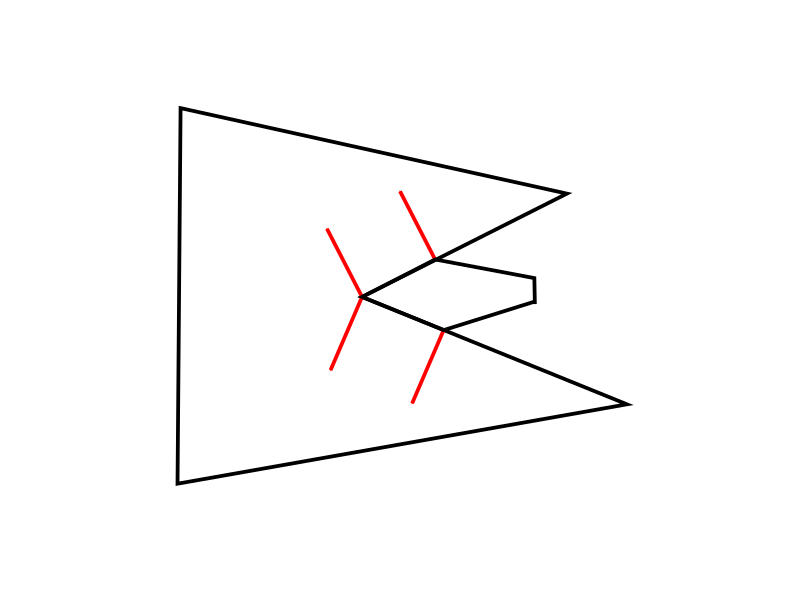
\includegraphics[width=0.45\textwidth]{images/4_contacts}
\par\end{centering}
\caption{4 non-immobilizing contacts.\label{fig:4-contacts}}
\end{figure}
Adding one finger to each object will immobilized it but the whole
configuration will no be immobilized having only 2 external contacts.
Assessment of such cases is discussed in\ref{sec:MultiO-eval-n-grasp-secur}.

\paragraph{Finding 2 contacts for a case of 2 given contacts or for a flat wrench
convex cone of 3+ contacts.}

\z{$O(n log(n))$ or $O(n^2)$ ? }Given 2 contacts, or 3 contacts that
form a flat wrench cone, additional contacts can be found be examining
wrench space vectors. For a case with 3 degenerate contacts, 2 marginal
vectors are selected. Wrench space vectors and the origin form a plane
(from now on``the plane''). Once such plane is determined, possible
complementary contacts can be tested. First, simple one-edge solutions
are proposed and evaluated. For each edge a corresponding generalized
wrench is built and tested to be on both sides of the plane. If such
edge found, two marginal wrenches are tested to get grasp quality
measure, which is saved along with contact locations.

\begin{algorithm}[H]
\label{alg:contacts34}
\caption{$\mathtt{c3\_c4\_for\_P\_given\_2c\_A}$}    % Determine the region for 4th contact given 3
\KwData{Polygon: $P$,  2 contacts: $C_{1},C_{2}$}
\KwResult{$CP_{34}$: a set of location pairs for 3rd and 4th contacts to form desired grasp}
	$w_1, w_2 =\mathrm{WrenchesOf}\left(C_1,C_2\right)$\;

\For{$e_i$ = edge of $P$}
	{
\If{ $\mathtt{span}\left\{\hat{n}_{C_{1}},\hat{n}_{C_{2}},\hat{n}_{e_{i}}\right\} =\rtwo $ }{

\tcc{Create a generalized wrench for the edge}
			$GW = GeneralizedWrench(e_i)$\;
\tcc{Find marginal wrenches of the generalized edge wrench}
			$w_a =\underset{w}{\mathrm{\min}}\left(GW\right)$\;
			$w_b =\underset{w}{\mathrm{\max}}\left(GW\right)$\;
\tcc{If marginal wrenches are on different sides of the plane formed by w3,w4}
\If{$\left(\left( w_1\times w_2\right)\times w_a\right)\cdot\left(\left( w_1\times w_2\right)\times w_b\right) < 0$}
			{
\tcc{If the wrenches are on different sides they will form a convex hull around the origin, save them as potential contacts}
				$GQM = GraspQualityMeasure\left(w_1, w_2, w_a,w_b\right) $\;
				$CP_{34}\twoheadleftarrow\{\mathtt{locationsFromWrenches}\left(w_a,w_b\right), GQM\} $\;
			}

		}
	}
\end{algorithm}

If no such edge found, or if higher quality measures are desired,
variants of 2 edge combinations are selected to check whether they
complete the convex hull of wrench vectors. Generalized wrenches are
built and for each pair assessed to have a components on opposite
sides of the plane. When such pair is found, corresponding regions
of the edges are valid places for finger placement. A selection of
contact locations can be done by extracting contact location from
wrenches that have largest grasp quality measure. The algorithm is
presented below:

\begin{algorithm}[H]
\label{alg:contacts34}
\caption{$\mathtt{c3\_c4\_for\_P\_given\_2c\_B}$}    % Determine the region for 4th contact given 3
\KwData{Polygon: $P$,  2 contacts: $C_{1},C_{2}$}
\KwResult{$CP_{34}$: a set of location pairs for 3rd and 4th contacts to form desired grasp}
	$w_1, w_2 =\mathrm{WrenchesOf}\left(C_1,C_2\right)$\;
	$\hat{n}_{plane12} = w_1\times w_2 $\;
\For{$e_i, e_j$ = edge pairs of $P$ 2-edge variants list}
	{
\If{ $\mathtt{span}\left\{\hat{n}_{C_{1}},\hat{n}_{C_{2}},\hat{n}_{e_{i}}\right\} =\rtwo $ }{
\tcc{Create a generalized wrench for each edge}
			$GW_i = GeneralizedWrench(e_i)$\;
			$GW_j = GeneralizedWrench(e_j)$\;
\uIf{ $GW_i$ is fully on one side of the plane }{
\tcc{Select first wrench the farthest from the plane}
				$w_a =\underset{w}{\argmax}\left|w\cdot\hat{n}_{plane12}\right|,\, w\in GW_i $\;
\tcc{Select second wrench the farthest from the plane from the other side}
				$w_b =\underset{w}{\argmax}\left|-\mathtt{sign}\left(w\cdot\hat{n}_{plane12}\right)w\cdot\hat{n}_{plane12}\right|,\, w\in GW_j $\;
				$GQM = GraspQualityMeasure\left( w_a,w_b\right) $\;
				$CP_{34}\twoheadleftarrow\{\mathtt{locationFromWrenches}\left(w_a,w_b\right), GQM\} $\;
			}
\Else{
\tcc{Both GW's are on both sides of the plane}
				$w_a =\underset{w}{\argmax}\left(\,w\cdot\hat{n}_{plane12}\right),\, w\in\{GW_i, GW_j\} $\;
				$w_b =\underset{w}{\argmax}\left(\,-w\cdot\hat{n}_{plane12}\right),\, w\in\{GW_i, GW_j\} $\;
\tcc{Select maximally distant wrench on each side}
				$GQM = GraspQualityMeasure\left(w_1, w_2, w_a,w_b\right) $\;
				$CP_{34}\twoheadleftarrow\{\mathtt{locationFromWrenches}\left(w_a,w_b\right), GQM\} $\;
			}
		}
	}
\end{algorithm}

\paragraph{Finding 3 finger contacts for 1 inter-object contact}

This case is the most undefined and require more decisions as to finger
placement locations. Some of the proposed methods for object immobilization
can be applied for this case with minor adjustments. The method presented
below is influenced by methods proposed by\citet{Wu2006} for IRC
evaluation and\citep{Nguyen1986a} compliance and grasp polygons.

First, we define a geometric 2 dimensional convex cone: a planar angle
between two vectors. The cone can be fully defined by a vertex point
and 2 vectors.Total force applied by 2 contacts can be defined to
lie in such cone that is formed by two contact normal directions.
This is analogous to friction cone of single frictional contact (see\citet{Nguyen1986}).
The main idea is to form 2 imaginary convex cones each formed by 2
normal vectors. The line connecting the cones' vertices should lie
inside of the intersection of 2 cones (or intersection of anti-cones
of these 2 cones). If the connecting line lies inside - the grasp
will be force closure. 

For given problem, one contact is given and non movable, other 3 can
be placed anywhere desired. Contact 2 is placed on arbitrary edge
in a position that ensures that the cone ($\triangleq ConeA$) formed
by it and so$ConeA$ will have the most area of intersection with
the polygon. Afterwards other edges tested to form a cone that will
have a common intersection with $ConeA$, and this way it will complete
the grasp. If there is no intersection between two cones, intersection
between anti-cones is tested.

Given a polygon with one inter-polygon contact:

Two variants of the algorithm presented, where first one is testing
simple combinations with lower computational complexity, and second
one is more robust but requires more computations.

\begin{algorithm}[H]
\label{alg:contacts234}
\caption{$\mathtt{c2,c3,c4\_for\_P\_given\_c\quad Variant\_A}\qquad$}    % Determine the region for 4th contact given 3
\KwData{Polygon: $P$, contact: $C_{1}$}
\KwResult{$CP_{234}$: a set of location triplets for 2nd, 3rd and 4th contacts to form desired grasp}

\For{$e_i$ = edge of $P$}{
		$ p =\mathtt{projection\_a\_on\_b\_along\_c}(e_i,\hat{n}_{C_1},\hat{n}_{e_i}) $\;
\For{$e_j$ = edge of $P$, $j\neq i$}{
\If{$\vec{0}\in ConvexHull\left(\hat{n}_{e_j},\hat{n}_{e_i},\hat{n}_{C_1}\right)  $}{
\tcc{The edge can possibly provide 2 contacts to form a force closure grasp.}
				$ p34 =\mathtt{proj\_a\_on\_b\_along\_c}(e_i,\hat{n}_{C_1},\hat{n}_{e_i}) $\;
				$ p2 =\mathtt{proj\_a\_on\_b\_along\_c}(p, e_j,\hat{n}_{e_j}) $\;
\If{$\left| p2\cup  p34\right| > 1 $} {
\tcc{The projections intersection is more than one point}
					$ m =\mathtt{mean}\left(p2\cup  p34\right) $\;
					$l_2 =\mathtt{proj\_a\_on\_b\_along\_c}(m, e_i,\hat{n}_{e_i})$\;
					$ s1,s2 =\mathtt{segment\_divided\_by\_point}\left(p34, m\right) $\;
					$l_3 =\mathtt{proj\_a\_on\_b\_along\_c}\left(\mathtt{mean}\left(s1\right), e_j,\hat{n}_{e_j}\right)$\;
					$l_4 =\mathtt{proj\_a\_on\_b\_along\_c}\left(\mathtt{mean}\left(s2\right), e_j,\hat{n}_{e_j}\right)$\;
					$GQM = GraspQualityMeasure\left(w_{C_1}, w_{l_2}, w_{l_3}, w_{l_4}\right) $\;
					$CP_{234}\twoheadleftarrow\{ l_2, l_3, l_4, GQM\} $\;
				}
			}
		}
	}
\end{algorithm}

If no suitable combinations found by the algorithm presented above,
following algorithm can be used:

\begin{algorithm}[H]
\label{alg:contacts234}
\caption{$\mathtt{c2,c3,c4\_for\_P\_given\_c\quad Variant\_B}\qquad$}    % Determine the region for 4th contact given 3
\KwData{Polygon: $P$, contact: $C_{1}$}
\KwResult{$CP_{234}$: a set of location triplets for 2nd, 3rd and 4th contacts to form desired grasp}

\For{$e_i$ = edge of $P$}{
		$ p =\mathtt{projection\_a\_on\_b\_along\_c}(e_i,\hat{n}_{C_1},\hat{n}_{e_i}) $\;
\For{$e_j$ = edge of $P$, $j\neq i$}{
\For{$e_k$ = edge of $P$, $k\neq i\;\mathrm{ and }\; k\neq j $}{
\If{$\vec{0}\in ConvexHull\left(\hat{n}_{e_i},\hat{n}_{e_j},\hat{n}_{e_k},\hat{n}_{C_1}\right)  $}{
\tcc{Since 3 edges along given contact can form a convex hull that containts the origin, we can proceed to determine preferred locations along these edges.}
					$ p_{e_i} =\underset{p\in e_i}{\argmin}\left(p\cdot\hat{n}_{C_1}\right)  $\;
					$ p_{e_j} =\underset{p\in e_j}{\argmin}\left(p\cdot\hat{n}_{e_k}\right)  $\;
					$ p_{e_k} =\underset{p\in e_k}{\argmin}\left(p\cdot\hat{n}_{e_j}\right)  $\;
\tcc{Find bounding points that yield maximum cone intersection area}
					$ v_1 = intersection\left( p_{C_1}+\hat{n}_{C_1}, p_{e_i}+\hat{n}_{e_i}\right) $\;
					$ v_2 = intersection\left( p_{e_j} +\hat{n}_{e_j}, p_{e_k}+\hat{n}_{e_k}\right) $\;
					$ConeA = ConvexCone\left(v=v_1, n_a =\hat{n}_{C_1}, n_b=\hat{n}_{e_i}\right)$\;
					$ConeB = ConvexCone\left(v=v_2, n_a =\hat{n}_{e_j}, n_b=\hat{n}_{e_k}\right)$\;
\If{$\left(v_1 - v_2\right)\in\left(ConeA\cap ConeB\right)\cup\left(-ConeA\cap -ConeB\right) $}{
\tcc{The line connecting cone vertices is inside the cone or anti-cone intersection means that the grasp is force closure / torque closure. Now contact locations can be selected.}
						$l_2 =\mathtt{proj\_a\_on\_b\_along\_c}\left(0.3\cdot\left(v_1 - v_2\right), e_i,\hat{n}_{e_i}\right)$\;
						$l_3 =\mathtt{proj\_a\_on\_b\_along\_c}\left(0.3\cdot\left(v_2 - v_1\right), e_j,\hat{n}_{e_j}\right)$\;
						$l_4 =\mathtt{proj\_a\_on\_b\_along\_c}\left(0.3\cdot\left(v_2 - v_1\right), e_k,\hat{n}_{e_k}\right)$\;
						$GQM = GraspQualityMeasure\left(w_{C_1}, w_{l_2}, w_{l_3}, w_{l_4}\right) $\;
						$CP_{234}\twoheadleftarrow\{ l_2, l_3, l_4, GQM\} $\;
					}
				}
			}
		}
	}
\end{algorithm}

Once all polygons are treated, desired contacts should be selected.
Since all contact positions are saved along with grasp quality measure
values, it is possible to select the contacts that provide better
grasp. While maintaining

Flowchart for object treatment given contacts.

What about a restrictions on finger placement that arise from close
objects? Should it be discussed and treated?? \#

\z{DEAL WITH THIS PART LATER}

\subsection{Completeness}

t

\subsection{Complexity}

t

\section{Multi object grasp evaluation and grasp securing\label{sec:MultiO-eval-n-grasp-secur}}

Once every given object is immobilized by other objects and fingers,
the constellation still might be not fully immobilized. Example:\ref{fig:2-of-3-objects-not-immobilized}
shows 3 objects: black object is immobilized by 4 contacts from red
and blue objects while red and and blue are immobilized by two additional
fingers each one. The contacts that act on blue and black objects
(shown as red arrows) intersect at same point and hence do not immobilize
these two objects together -- namely, these two objects can rotate
together about the contact intersection point.
\begin{figure}[tbh]
\noindent \begin{centering}
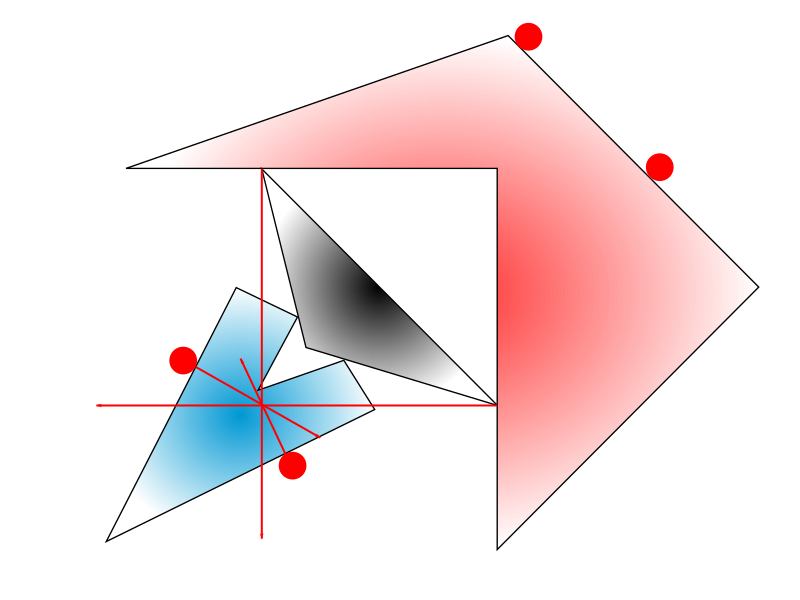
\includegraphics[width=0.45\textwidth]{images/constellation_evaluation}
\par\end{centering}
\caption{2 of 3 objects are not immobilized.\label{fig:2-of-3-objects-not-immobilized}}
\end{figure}
Total immobilization can be achieved by ensuring that every possible
subset of objects is immobilized. This requires extraction of all
possible connected subsets from the given set object and evaluation
whether they are or are not immobilized. Each constellation ought
to have at least 4 external contacts. If there are less - additional
contacts required to immobilize it.
\begin{figure}[tbh]
\noindent \begin{centering}
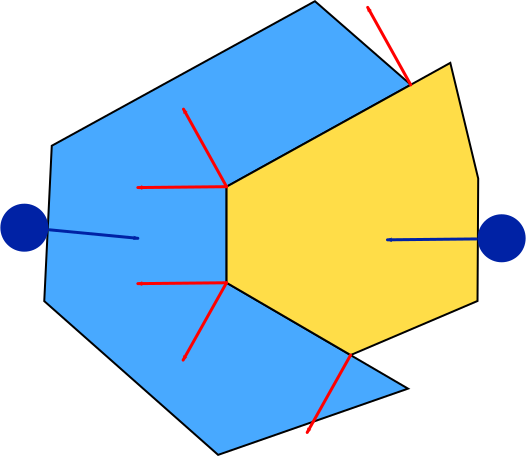
\includegraphics[width=0.3\textwidth]{images/not_immobilized_object_set}
\par\end{centering}
\caption{2 objects set is not immobilized.}
\end{figure}
If the amount of external contacts is higher than 4, assessment of
intersection of contacts external to the subset can show whether the
subset is immobilized or not. If the contacts intersect at one point,
contact positions of added fingers can be altered in a allowed regions
that were found for that contact. 

\begin{algorithm}[H]
\caption{Multi object grasp evaluation}   
\KwData{Set of polygons $P = {p_i}\;i\in \left[ 1,K \right]$ including locations and orientations, Set of contacts $C = \left\{c_i\right\}$ with allowed regions}
\KwResult{Set of contact adjustments if needed, set of additional contacts if needed }
\ForEach{subset of object configuration}
{
	L = $\left\{lc_i\right\}$ -- set of external contact lines\;
	\If{$\left| L \right| < 4$}
	{
		Treat the subset as one object\;
		\If{$\left| L \right| = 3 $ and $ \exists\, x \in lc_i\quad \forall lc_i \in L $}
		{
			Move 1 finger in allowed region\;
		}
		Add missing contacts (max 2)\;
	}
%%	N = $\left\{nc_i\right\}$ -- set of normal directions of external contacts\;
	\uIf{$ \exists\, x \in lc_i\quad \forall lc_i \in L $}
	{
		Intersection point between contact lines exists\;
		Build 2 EGWs for 2 non-collinear contacts and adjust positions\;
	}
	\uElseIf{$ \exists\, x_1 \in lc_j\quad j={1,2,3} $}
	{	
		3 of the contacts are intersecting\;
		\If{$ \exists\, x_2 \in lc_k , \notin lc_j\quad \left|\left\{lc_k\right\}\right|>1$}
		{
			Exists another point where two or more contact lines intersect\;
			\textbf{\textit{continue}}\;
		}
		Build 2 EGWs for 2 non-collinear $lc_j$ and adjust positions\;
	}
	\Else
	{
		\textbf{\textit{continue}}\;
	}	
]



}
\end{algorithm}

\section{Objects rearrangement}

Once desired configuration is found the rearrangement planning is
needed. Many algorithms for single object manipulations were developed,
but in this case due to several objects to be moved. Objects placement
algorithms are designed in a way that will allow stacking the objects
in the defined order.

Objects can be moved individually by executing any planning algorithm
for single object.\citet{Akella1998,Bernheisel2004,Lynch1992,Lynch1999}
present methods for moving objects in assemblies in plane. Simultaneous
manipulation of several objects is out of the scope of this research,
and it is assumed that there is a way to rearrange the objects from
given configuration to the desired one.

For the purposes of simulations and experiments, objects are scattered
in the workspace at distances that allow for each object to be repositioned
at desired location. Each manipulation is defined by base object and
moved object. Objects are grasped and moved individually while maintaining
finger positions that will not interfere with adjacent objects. Alternatively,
if no such option exists, the object can be positioned at a pre-pose
and pushed from there.

\z{Should I mention this ?:} Objects are moved by stable pushing
which allows translation and rotation of the object. Geometric center
assumed to be the center of rotation.

Base object is an object or a set of objects that serve as a base
for a moved object to be placed in contact to.

\section{Complexity}

\z{What in hell do I write here?}

\section{Limitations}

\z{What can I write here?}

Limitations of the finger placement? Finger sizes, proximity to the
vertex -- dealing with uncertainty. While rearranging:

Limitation of the multiobject evaluation? Object placement?

Quality measure contradictions: what's best for one polygon not necessary
is best for polygon constellation.

\chapter{Results}

The chapter presents the results of the algorithms performance.\z{Duh!}

\section{Simulations}

Geometrical simulations were performed in MATLAB environment. The
simulations included assessment of polygonal objects, rearrangement
algorithm evaluations and finger placement algorithms execution. The
obtained results are tested for consistency, and mathematically assessed
for the completeness of the solution. Several methods are compared
and comparison results are presented.

\subsection{Software}

MATLAB computing environment was used for the purpose of geometrical
simulations. Specialized graphical user interface (GUI) programs were
created for evaluation and presentation of the algorithms\footnote{The programs are available at\href{https://github.com/yossioo/MSc-Research}{https://github.com/yossioo/MSc-Research}.}.

\subsection{Setup}

V-REP environment was used for physical simulation of the performance
of the algorithms. The software incorporated several common physics
engines which allow testing of different scenarios of computer simulations.

Delta-robot model of \&\& was used to perform as the main manipulator,
custom end effector was added to the model to perform grasping of
desired object sets.

The end-effector consists of 10 individually actuated fingers, which
can move in the``palm'' plane freely and have limited movement in
Z direction. Depending on the found solution, the desired number of
fingers can be extended to execute the grasp.

Objects' location and orientation is obtained programmatically, while
in real life scenario can be done by different means (e.g. RGB or
3D cameras, tracking cameras, resistive or capacitive surfaces etc.)

Control of the robot is done in closed loop by internal means of the
V-REP software, while the control of the algorithm steps is done in
the specialized GUI. The simulation is divided into several steps:
\begin{enumerate}
\item Obtaining environment information:
\begin{enumerate}
\item Number of objects
\item Positions
\item Shapes
\end{enumerate}
\item Obtaining the desired constellation variants
\begin{enumerate}
\item variants are shown in preview pane along with quality measures
\item desired variant can be selected for the execution
\end{enumerate}
\item Rearranging the objects
\begin{enumerate}
\item objects are moved by pushing algorithms to obtain the desired configuration
\end{enumerate}
\item Immobilizing the objects
\begin{enumerate}
\item Required amount of fingers are selected and extended to perform the
grasp
\item manipulator moves above the objects
\item Manipulator and the end effector are lowered down to constrain the
constellation
\end{enumerate}
\item Immobilization tests
\begin{enumerate}
\item moving in plane
\item moving to vertical plane and rotating
\end{enumerate}
\end{enumerate}
Executions of the steps can be controlled from the UI.

\subsection{Results}

A simple case of 3 equilateral triangles presented in the \emph{SIMULATIONS.
The designed configuration and designed grasp are presented above.
3D printed end effector is presented on the FIGURE. Due to }

A case of 6 equilateral triangles

A case of 3 squares

A case of 4 squares

A case of 3 hexagons

Cases of 3-4-5-... irregular triangles.

A case of 3-4-5 octagons?

\section{Experiments}

Bring a 3D printed set of objects and designed gripper to the defense.
Include the results in the Appendix, and in the presentation

The results of the algorithms' performance were tested in experimental
setups. Robotic manipulator with 6DOF was equipped with an end effector
designed according to the algorithm's output. The robot is controlled
by a laptop with Robot Operating System (ROS) hosted in Ubuntu. Several
polygonal objects were selected to be stacked, and after the verification
by the algorithm a custom-made end effector with stationary fingers
was manufactured by 3D printing. The end effector was tested and confirmed
to immobilize the desired set of objects both in simulation and in
experiments. Due to the real world imperfections, the fingers of the
designed end effectors are made with chamfers, this allowed grasping
of the arranged set of items despite small perturbations of item locations
and robotic arm performance.

\subsection{Experimental Setup}

For several examined cases of polygon sets, 

\subsection{Experimental Results}

A simple case of 3 equilateral triangles presented in the SIMULATIONS.
The designed configuration and designed grasp are presented above.
3D printed end effector is presented on the FIGURE. Fingers - 1 joint
finger - touches 2 triangles.

A case of 6 equilateral triangles

A case of 3 hexagons

Cases of 3-4-5-... irregular triangles.

\chapter{Discussion}

Written before Conclusions

\chapter{Conclusions}

Written before the Introduction

\newpage{}

\bibliographystyle{apalike}
\phantomsection\addcontentsline{toc}{chapter}{\bibname}\bibliography{main}


\appendix

\chapter*{Appendix}

\chapter{Algorithms}

This section presents more elaborate representation of the algorithms
presented in the paper.

\chapter{Software}

Source code is available at\href{https://github.com/yossioo/MSc-Research}{https://github.com/yossioo/MSc-Research}.

Additional videos are available at Youtube channel: \&\&\&

The software used for the research is:

MATLAB r2018a

V-REP 3.5.0 Educational Version

ROS Kinetic on Ubuntu 16.04

\chapter{Examples of calculated grasps}

3 fingers - 1 found

\chapter{Examples of rearranged object sets}

\chapter{Examples of finger combinations found for sets}

\chapter{Simulations}

V-REP

\chapter{Experiments}

Real robot


\chapter{Junk}

\begin{tikzpicture}
\draw (0,0) to [R=1<\kilo\ohm>]
(3,0) to [ I , i=50<\milli\ampere>]
(6,0) to [R=516<\ohm>]
(6,3) to [V,v=50<V>]
(3,3) to [diode ]
(0,3) to [ ospst=S]
(0,0);
\end{tikzpicture}

\begin{figure}[tbh]
\begin{centering}
\smartdiagram[descriptive diagram]{
  {Style,{Define shapes, colors, shading,
          and line styles for nodes and arrows}},
  {Position, {Place nodes using a matrix,
              relative or absolute positioning}},
  {Relation, Insert edges or arrows
             between selected nodes},
  {Label, Add labels on edges or arrows}}\begin{center}
\begin{tikzpicture}
\begin{scope}[blend group = soft light]
\fill[red!30!white]   ( 90:1.2) circle (2);
\fill[green!30!white] (210:1.2) circle (2);
\fill[blue!30!white]  (330:1.2) circle (2);
\end{scope}
\node at ( 90:2)    {Typography};
\node at ( 210:2)   {Writing};
\node at ( 330:2)   {Coding};
\node [font=\Large] {\LaTeX};
\end{tikzpicture}
\par\end{center}
\par\end{centering}
\caption{222}
\end{figure}

-----------

\begin{tikzpicture}
\begin{axis}
[grid=major,samples=100,mark=none]
\addplot[red,very thick ,domain=-180:180]{x*sin(x)};
\end{axis}
\end{tikzpicture}

XY example

\[
\xymatrix{\text{Some text here}\ar[dr] & \cos\left(\theta\right) & e\\
c\ar[ur]\ar[rr]_{Under}^{Over} &  & f
}
\]

\end{document}
